\documentclass[a4paper]{report}

\def\baselinestretch{1.1}
\usepackage[14pt]{extsizes}
\usepackage[utf8]{inputenc}
\usepackage{listings}
\usepackage{xcolor} % Для работы с цветами
\usepackage[english, russian]{babel}
\usepackage{indentfirst}
\usepackage{mathrsfs}


%%%%%%%%%%%%%%%%% Символы, графика %%%%%%%%%%%%%%%%%%%%%

\usepackage[T1,T2A]{fontenc}
\usepackage{amsmath,amssymb,amsfonts,amsthm}
\usepackage{bm}
\newcommand\dsone{\mathds{H}}
\usepackage{graphicx}
\usepackage{color}
\usepackage[pdftex,colorlinks,linkcolor=blue,citecolor=blue]{hyperref}
\usepackage{pgfplots}
\usepackage{tikz}
\usetikzlibrary{through, shapes, snakes}
\usepackage{array}
\usepackage{algorithm}
\usepackage{algcompatible}
\newcolumntype{P}[1]{>{\centering\arraybackslash}p{#1}}

%%%%%%%%% Разметка страницы %%%%%%%%%

\bibliographystyle{plain}  % Change this to your preferred style
\renewcommand{\thetable}{\arabic{table}}
\usepackage{indentfirst}
\usepackage{tocloft}
\topmargin=-1.4cm %отступ сверху
\oddsidemargin=0.4cm %отступ слева (нечетные страницы)
\evensidemargin=0.4cm %(четные страницы)
\textwidth=16cm %ширина текста
\textheight=24cm
\tolerance=800
\parskip=0.8ex

\pagestyle{plain}

\definecolor{background}{RGB}{248, 248, 248}
\definecolor{string}{RGB}{246, 102, 30}
\definecolor{comment}{RGB}{0, 128, 1}
\definecolor{normal}{RGB}{0, 0, 0}
\definecolor{identifier}{RGB}{0, 150, 186}
\definecolor{keyword}{RGB}{138, 49, 185}
\definecolor{variables}{RGB}{229, 8, 118}

% Основные настройки для поддержки кириллицы
\lstset{
    alsoletter=.,
    language=python,                			% choose the language of the code
    numbers=left,                   		% where to put the line-numbers
    stepnumber=1,                   		% the step between two line-numbers.
    numbersep=5pt,                  		% how far the line-numbers are from the code
    numberstyle=\tiny\color{black}\ttfamily,
    backgroundcolor=\color{background},  		% choose the background color. You must add \usepackage{color}
    showspaces=false,               		% show spaces adding particular underscores
    showstringspaces=false,         		% underline spaces within strings
    showtabs=false,                 		% show tabs within strings adding particular underscores
    tabsize=4,                      		% sets default tabsize to 2 spaces
    captionpos=b,                   		% sets the caption-position to bottom
    breaklines=true,                		% sets automatic line breaking
    breakatwhitespace=true,         		% sets if automatic breaks should only happen at whitespace
    title=\lstname,                 		% show the filename of files included with \lstinputlisting;
    basicstyle=\color{normal}\ttfamily\footnotesize,					% sets font style for the code
    keywordstyle=\color{keyword}\textbf,	% sets color for keywords
    stringstyle=\color{string}\ttfamily,		% sets color for strings
    commentstyle=\color{comment}\ttfamily,	% sets color for comments
    emph={
    print, input, open, close, read, write,
    len, range, enumerate, zip, format, split, join,
    print_pauli_table, get_base_path, console_and_print, ljust, rstrip,
    create_table, format_ansatz, format_complex_number,
    format_number, get_operator_for_console, initialize_environment,
    print_composition_table, print_hamiltonian, print_pauli_table,
    read_file_lines, read_hamiltonian_data, generate_random_theta,
    multiply_pauli, pauli_compose, calculate_ansatz, compute_uhu,
    calculate_expectation, generate_neighbor_theta, simulated_annealing,
    main, getattr,  print_composition_table, generate_shifted_theta
    },
    emphstyle=\color{identifier}\ttfamily,
    mathescape=true,
    literate=
        {π}{{$\pi$}}1
        {±}{{$\pm$}}1
        {θ}{{$\theta$}}1
        {σ}{{$\sigma$}}1
        {·}{{$\cdot$}}1
        {₁}{{\textsubscript{1}}}1
        {₂}{{\textsubscript{2}}}1
        {…}{{\cdots}}1
        {→}{{$\rightarrow$}}1
        {†}{{\textdagger}}1
        {а}{{\cyra}}1
        {б}{{\cyrb}}1
        {в}{{\cyrv}}1
        {г}{{\cyrg}}1
        {д}{{\cyrd}}1
        {е}{{\cyre}}1
        {ё}{{\"e}}1
        {ж}{{\cyrzh}}1
        {з}{{\cyrz}}1
        {и}{{\cyri}}1
        {й}{{\cyrishrt}}1
        {к}{{\cyrk}}1
        {л}{{\cyrl}}1
        {м}{{\cyrm}}1
        {н}{{\cyrn}}1
        {о}{{\cyro}}1
        {п}{{\cyrp}}1
        {р}{{\cyrr}}1
        {с}{{\cyrs}}1
        {т}{{\cyrt}}1
        {у}{{\cyru}}1
        {ф}{{\cyrf}}1
        {х}{{\cyrh}}1
        {ц}{{\cyrc}}1
        {ч}{{\cyrch}}1
        {ш}{{\cyrsh}}1
        {щ}{{\cyrshch}}1
        {ъ}{{\cyrhrdsn}}1
        {ы}{{\cyrery}}1
        {ь}{{\cyrsftsn}}1
        {э}{{\cyrerev}}1
        {ю}{{\cyryu}}1
        {я}{{\cyrya}}1
        {А}{{\CYRA}}1
        {Б}{{\CYRB}}1
        {В}{{\CYRV}}1
        {Г}{{\CYRG}}1
        {Д}{{\CYRD}}1
        {Е}{{\CYRE}}1
        {Ё}{{\CYRYO}}1
        {Ж}{{\CYRZH}}1
        {З}{{\CYRZ}}1
        {И}{{\CYRI}}1
        {Й}{{\CYRISHRT}}1
        {К}{{\CYRK}}1
        {Л}{{\CYRL}}1
        {М}{{\CYRM}}1
        {Н}{{\CYRN}}1
        {О}{{\CYRO}}1
        {П}{{\CYRP}}1
        {Р}{{\CYRR}}1
        {С}{{\CYRS}}1
        {Т}{{\CYRT}}1
        {У}{{\CYRU}}1
        {Ф}{{\CYRF}}1
        {Х}{{\CYRH}}1
        {Ц}{{\CYRC}}1
        {Ч}{{\CYRCH}}1
        {Ш}{{\CYRSH}}1
        {Щ}{{\CYRSHCH}}1
        {Ъ}{{\CYRHRDSN}}1
        {Ы}{{\CYRERY}}1
        {Ь}{{\CYRSFTSN}}1
        {Э}{{\CYREREV}}1
        {Ю}{{\CYRYU}}1
        {Я}{{\CYRYA}}1,
}


%%%%%%%% newcommands:  ket,  bra,  ketbra,  braket
\newcommand{\ket}[1] {\!\!\;\ensuremath{\left|#1\right\rangle}}
\newcommand{\bra}[1] {\!\!\:\ensuremath{\left\langle#1\right|\!\!\:}}
\newcommand{\ketbra}[2]{\!\!\:\ensuremath {\left|#1\right\rangle\!\:\!\!\left\langle#2\right|}}
\newcommand{\braket}[2]{\ensuremath {\!\!\:\left\langle#1\!\!\: \left|\!\!\!\;\right.#2\right\rangle\!\!\;}}

\begin{document}

\begin{titlepage}
	\begin{center}
		Министерство науки и высшего образования РФ\\
		ФГБОУ ВО «Тверской государственный университет»\\
		Математический факультет\\
		Направление 02.04.01 Математика и компьютерные науки\\
		Профиль <<Математическое и компьютерное моделирование>>	
	\end{center}
	
	\vspace{1.4cm}
	\begin{center}
	
		{МАГИСТЕРСКАЯ ДИССЕРТАЦИЯ}	
		
		\vspace{1.0cm}
    \large{Вариационный квантовый алгоритм с оптимизацией методом отжига}
		
		
		\vspace{1.0cm}
	\end{center}
	
	
	
	\begin{flushright}
		\begin{minipage}{80mm}
			Автор:\\
			Алешин Д.А.\\
      Подпись:
			
			\vspace{1.0cm}
			Научный руководитель:\\
			д. ф.-м. н. Цирулёв А.Н.\\
      Подпись:
			
		\end{minipage}
	\end{flushright}
	
	
	\vspace{1.6cm}
	\noindent Допущен к защите:\\
	Руководитель ООП: Цветков В.П.\\[0.3cm]
  $\underset{\textit{(подпись, дата)}}{\underline{\hspace{0.3\textwidth}}}$
	\vspace{2.2cm}
	
	
	
	\begin{center}
		Тверь 2025
	\end{center}
	
	\date{}
\end{titlepage}

\setcounter{page}{2}
\addtocontents{toc}{\protect\vspace{-6ex}}
\tableofcontents
\newpage

% Abstract
\addcontentsline{toc}{chapter}{\hspace{5.5mm} Введение}
\chapter*{Введение}

В последние годы вариационные квантовые алгоритмы приобретают всё большее значение в современных исследованиях по математическому моделированию и квантовым вычислениям. Особый интерес представляют гибридные квантово-классические методы, в которых оптимизация параметров квантовых схем сочетается с классическими алгоритмами поиска минимума. Такие подходы позволяют эффективно моделировать и исследовать малоразмерные квантовые системы, актуальные для описания новых состояний вещества, включая топологические материалы~\cite{Cerezo2021}.

Важной прикладной задачей в области вариационных квантовых алгоритмов является поиск основного состояния гамильтониана, что эквивалентно задаче минимизации средней энергии в пространстве квантовых состояний, генерируемых параметризованным анзацем. На практике решение такой задачи требует эффективных методов оптимизации, устойчивых к наличию большого числа локальных минимумов и не требующих вычисления производных целевой функции. Среди таких методов особое место занимает метод имитации отжига, который широко используется в задачах глобальной оптимизации и хорошо адаптируется к вариационным квантовым схемам.

Целью данной работы является построение и исследование вариационного квантового алгоритма с классической оптимизацией методом имитации отжига для поиска основного состояния гамильтониана квантовой системы.

В рамках исследования были поставлены следующие основные задачи:
\begin{enumerate}
    \item Изучить теоретические основы вариационных квантовых алгоритмов, включая формализм базиса Паули и построение анзаца для многокубитных систем;
    \item Разработать и реализовать алгоритм вариационной квантовой оптимизации с использованием метода имитации отжига;
    \item Провести сравнительный анализ эффективности различных параметров отжига и схем построения анзаца;
    \item Реализовать программную модель алгоритма на языке Python для практического моделирования процесса вариационной оптимизации.
\end{enumerate}

Объектом исследования является задача минимизации энергии гамильтониана в пространстве состояний, порождённых вариационным анзацем в базисе Паули. Предметом исследования выступает разработка и программная реализация гибридного квантового алгоритма с классическим оптимизатором на методе имитации отжига.

Структура работы включает две основные главы. В первой главе изложены теоретические основы вариационных квантовых алгоритмов, формализм базиса Паули и вопросы построения параметризованного анзаца. Вторая глава посвящена описанию метода имитации отжига, его адаптации к задачам квантовой оптимизации и программной реализации алгоритма, а также анализу результатов тестирования. В заключении приведены основные выводы по проделанной работе. Список литературы включает современные публикации российских и зарубежных авторов, посвящённые тематике квантовых вычислений и оптимизации.

В работе везде принята система единиц, в которой постоянная Планка $\hbar=1$ и скорость света $c=1$, что соответствует общепринятому подходу в теоретической физике.


\chapter{Общая схема квантовых вариационных алгоритмов}

\section{Базис Паули}
\subsection{Связь стандартного базиса и базиса \mbox{Паули}}

Рассмотрим квантовую систему из ${n}$ кубитов, где каждый кубит связан с двумерным гильбертовым пространством ${\mathcal{H}}$ и его эрмитово сопряжённым пространством ${\mathcal{H}^\dagger}$. Обозначим через ${\mathcal{H}_n = \mathcal{H}^{\otimes n}}$ и ${\mathcal{H}_n^\dagger = (\mathcal{H}^\dagger)^{\otimes n}}$ гильбертово пространство системы и его эрмитово сопряжение соответственно. Пространство линейных операторов, действующих на ${\mathcal{H}}$ и ${\mathcal{H}^\dagger}$ левым и правым умножением, задаётся как ${L(\mathcal{H}_n) = \mathcal{H}_n \otimes \mathcal{H}_n^\dagger}$. Тогда

$${\dim_\mathbb{C} \mathcal{H}_n = \dim_\mathbb{C} \mathcal{H}_n^\dagger = 2^n,\;\;\;
            \dim_\mathbb{C} L(\mathcal{H}_n) = 2^{2n}.}$$

Пространство ${L(\mathcal{H}_n)}$ наделено скалярным произведением Гильберта-Шмидта:

\begin{equation}\label{eq1}
    \langle\hat{A},\hat{B}\rangle = \mathrm{tr}(\hat{A}^\dagger\hat{B}),\;\;\;
    \hat{A},\hat{B} \in L(\mathcal{H}_n),
\end{equation}

\noindent которое естественно продолжает скалярное произведение в ${\mathcal{H}_n}$. Вещественное линейное пространство эрмитовых операторов далее обозначим как ${H(\mathcal{H}_n)}$.


Пусть ${\{|0\rangle,|1\rangle\}}$ образуют ортонормированный базис в однокубитном пространстве ${\mathcal{H}}$. Единичная матрица и матрицы Паули задаются как:

$${
    \sigma_0 = \begin{pmatrix}1 & 0 \\ 0 & 1\end{pmatrix},\;
    \sigma_1 = \begin{pmatrix}0 & 1 \\ 1 & 0\end{pmatrix},\;
    \sigma_2 = \begin{pmatrix}0 & -i \\ i & 0\end{pmatrix},\;
    \sigma_3 = \begin{pmatrix}1 & 0 \\ 0 & -1\end{pmatrix},
}$$

\noindent а соответствующие операторы Паули представляются в виде:
\begin{align*}
    \hat{\sigma}_0 = |0\rangle\langle0| + |1\rangle\langle1|,\;
    \hat{\sigma}_1 = |0\rangle\langle1| + |1\rangle\langle0|,     \\
    \hat{\sigma}_2 = -i|0\rangle\langle1| + i|1\rangle\langle0|,\;
    \hat{\sigma}_3 = |0\rangle\langle0| - |1\rangle\langle1|.
\end{align*}

\noindent Эти операторы одновременно эрмитовы и унитарны, а также образуют базис в ${\mathcal{H}}$. Обратное преобразование выражается следующим образом:

$${
    |0\rangle\langle0| = \frac{\hat{\sigma}_0 + \hat{\sigma}_3}{2},\;
    |0\rangle\langle1| = \frac{\hat{\sigma}_1 + i\hat{\sigma}_2}{2},\;
    |1\rangle\langle0| = \frac{\hat{\sigma}_1 - i\hat{\sigma}_2}{2},\;
    |1\rangle\langle1| = \frac{\hat{\sigma}_0 - \hat{\sigma}_3}{2}.
}$$

Для ${k, l, m \in \{1,2,3\}}$ выполняются свойства:
${\mathrm{tr}\hat{\sigma}_k = 0}$,
${\hat{\sigma}^2_k = \hat{\sigma}_0}$, а также

\begin{equation}\label{eq2}
    \hat{\sigma}_k\hat{\sigma}_l = -\hat{\sigma}_l\hat{\sigma}_k, \;\;\;
    \hat{\sigma}_k\hat{\sigma}_l = i\,\mathrm{sign}(\pi)\hat{\sigma}_m, \;\;\;
    (klm) = \pi(123),
\end{equation}

\noindent где ${\pi(123)}$ — произвольная перестановка множества ${\{1,2,3\}}$.

Рассмотрим стандартный\footnote[1]{Мы избегаем термина <<вычислительный>>, так как он может приводить к неоднозначности. И базис Паули, и стандартный базис являются вычислительными в одинаковом контексте.} бинарный базис в ${\mathcal{H}_n}$, образованный ортонормированными базисами ${\{|0\rangle,|1\rangle\}}$ в однокубитных пространствах. Позиция в тензорном произведении позволяет различать кубиты. Для фиксированного ${n}$ элементы этого базиса и соответствующие им элементы двумерного базиса удобно записывать как:
$${
    |k\rangle = |k_1\ldots k_n\rangle = |k_1\rangle \otimes \ldots \otimes |k_n\rangle,\;\;\;
    \langle k| = \langle k_1\ldots k_n| = \langle k_1|\otimes\ldots\otimes\langle k_n|,
}$$
\noindent где строки ${k_1\ldots k_n}$ (${k_1,\ldots,k_n\in\{0, 1\}}$) интерпретируются как двоичные числа с десятичным представлением ${k}$. Например, ${|101\rangle = |5\rangle}$ и ${|00110\rangle = |6\rangle}$.

В стандартном базисе:
$${
    |u\rangle = \sum_{k=0}^{2^n - 1} u_k |k\rangle, \;\;\;
    \hat{A} = \sum_{k,l=0}^{2^n - 1} a_{kl} |k\rangle\langle l|,
}$$
\noindent где ${|u\rangle \in \mathcal{H}_n}$ и ${\hat{A} \in L(\mathcal{H}_n)}$.

Базис Паули ${P(\mathcal{H}_n)}$ в ${L(\mathcal{H}_n)}$ определяется как:
\begin{equation}\label{eq3}
    \{\hat{\sigma}_{k_1\ldots k_n}\}_{k_1,\ldots,k_n\in\{0,1,2,3\}},\;\;\;
    \hat{\sigma}_{k_1\ldots k_n} = \hat{\sigma}_{k_1}\otimes\ldots\otimes\hat{\sigma}_{k_n},
\end{equation}
\noindent где ${\hat{\sigma}_{0\ldots 0}}$ — тождественный оператор. Базис ${P(\mathcal{H}_n)}$ содержит ${4^n}$ элементов. Для краткости будем использовать обозначение:
$${
    \hat{\sigma}_K = \hat{\sigma}_{k_1\ldots k_n},
}$$
\noindent где строка Паули ${k_1\ldots k_n}$ (${k_1,\ldots,k_n \in \{0,1,2,3\}}$) соответствует числу ${K}$ в десятичной системе (${0 \leq K \leq 4^n - 1}$). Строка Паули ${K}$ и элемент ${\hat{\sigma}_K}$ взаимно однозначно соответствуют друг другу.

Сравним ${P(\mathcal{H}_n)}$ со стандартным базисом. Для элементов базиса Паули выполняются:
\begin{equation}\label{eq4}
    \hat{\sigma}_{k_1\ldots k_n} \hat{\sigma}_{k_1\ldots k_n} = \hat{\sigma}_{0\ldots 0}, \;\;\;
    \mathrm{tr}\,\hat{\sigma}_{0\ldots 0} = 2^n,\;\;\;
    \mathrm{tr}\,\hat{\sigma}_{k_1\ldots k_n}\Big|_{k_1\ldots k_n \neq 0\ldots0} = 0.
\end{equation}

Базис Паули является эрмитовым, унитарным и ортогональным относительно скалярного произведения \eqref{eq1}. Отметим, что оператор ${|k\rangle\langle l|}$ из стандартного базиса не является унитарным или эрмитовым при ${k \neq l}$. Стандартный базис не включает тождественный оператор, который в этом базисе записывается как:
$${
    \sum_{k=0}^{2^n-1} |k\rangle \langle k|.
}$$

В базисе Паули любой оператор ${\hat{U}}$ из унитарной группы ${U(\mathcal{H}_n)}$ (где $\hat{U}^\dagger\hat{U} = \hat{\sigma}_{0\ldots0}$) раскладывается в виде:
$${
    \hat{U} = \sum_{i_1,\ldots,i_n\in\{0,1,2,3\}} U_{i_1\ldots i_n}\hat{\sigma}_{i_1\ldots i_n},\;\;\;
    \hat{U}^\dagger = \sum_{i_1,\ldots,i_n\in\{0,1,2,3\}} \overline{U}_{i_1\ldots i_n}\hat{\sigma}_{i_1\ldots i_n},
}$$
где коэффициенты удовлетворяют условиям:
$${
    \sum_{i_1,\ldots,i_n\in\{0,1,2,3\}} \overline{U}_{i_1\ldots i_n}U_{i_1\ldots i_n} = 1,\;\;\;
    \sum_{\substack{
        i_1,\ldots,i_n,j_1,\ldots,j_n\in\{0,1,2,3\} \\
        (i_1,\ldots,i_n)\neq(j_1,\ldots,j_n)
    }} \overline{U}_{i_1\ldots i_n}U_{j_1\ldots j_n} = 0.
}$$

Последнее условие эквивалентно ${2^{2n-1}(2^n-1)}$ независимым соотношениям.

Эрмитовы операторы в базисе Паули разлагаются с вещественными коэффициентами.


\subsection{Коммутационное и антикоммутационное соотношение}

Коммутатор определяет взаимодействие операторов при их перестановке. Для операторов ${A}$ и ${B}$ он задаётся как:
$${[A, B] = AB - BA.}$$

\noindent Если ${[A, B] = 0}$, операторы коммутируют; в противном случае — нет. В базисе Паули коммутаторы выражаются через символ Леви-Чивиты ${\varepsilon_{ijk}}$:
$${[\sigma_i, \sigma_j] = 2i\varepsilon_{ijk}\sigma_k,}$$

\noindent где ${\varepsilon_{ijk}}$ равен $1$ при чётной перестановке индексов ${(i,j,k)}$, $-1$ при нечётной и $0$ в остальных случаях. Например:
$${[\sigma_1, \sigma_2] = 2i\sigma_3,\;\;\; [\sigma_2, \sigma_3] = 2i\sigma_1.}$$

Антикоммутатор характеризует симметричное произведение операторов:
$${\{A, B\} = AB + BA.}$$

\noindent Если ${\{A, B\} = 0}$, операторы антикоммутируют. Для операторов Паули:
$${\{\sigma_i, \sigma_j\} = 2\delta_{ij},}$$

\noindent где ${\delta_{ij}}$ — символ Кронекера ($1$ при ${i = j}$, $0$ иначе). Примеры:
$${\{\sigma_1, \sigma_2\} = 0,\;\;\; \{\sigma_2, \sigma_3\} = 0.}$$

Коммутаторы и антикоммутаторы применяются в квантовой механике для анализа свойств систем (спин электрона, кубиты), в квантовой теории поля (взаимодействия частиц) и квантовых вычислениях (алгоритмы, коррекция ошибок). Коммутаторы помогают определить совместную измеримость наблюдаемых, а антикоммутаторы — описать фермионные системы.

%##################### Третий параграф первой главы ###############################

\subsection{Коммутирующие элементы в алгебре Ли группы ${SU(2^{n})}$}

Рассмотрим базис Паули и множество строк Паули длины ${n}$:
$${
    \mathrm{Str}_n = \{K = k_1\ldots k_n\}_{k_1,\ldots,k_n \in \{0,1,2,3\}}.
}$$

1. Множество ${\mathbb{F}_4 = \{0,1,2,3\}}$ образует квадгруппу ${\mbox{Клейна}}$ с умножением:
$${
    0 \cdot k = k,\;\;\;
    k \cdot k = 0,\;\;\;
    k \cdot l = m,
}$$
где ${k,l,m \in \{1,2,3\}}$ и ${(klm)}$ — произвольная перестановка ${(1\,2\,3)}$.

2. Функция ${s: \mathbb{F}_4 \times \mathbb{F}_4 \to \{1, i, -i\}}$ задаётся значениями:
$${
    \begin{array}{ll}
        s(0,0) = s(0,k) = s(k,0) = s(k,k) = 1, & k=1,2,3, \\
        s(1,2) = s(2,3) = s(3,1) = i, & s(2,1) = s(3,2) = s(1,3) = -i.
    \end{array}
}$$

3. Функция ${S: \mathrm{Str}_n \times \mathrm{Str}_n \to \{1, -1, i, -i\}}$ определяется как:
$${
    S_{KL} = s(k_1, l_1) \cdot s(k_2, l_2) \cdot \ldots \cdot s(k_n, l_n),
}$$
где ${K = k_1k_2\ldots k_n}$ и ${L = l_1l_2\ldots l_n}$.

Симметрия функции ${S}$ зависит от числа пар ${(k_r, l_r)}$ (на позициях ${r}$ в строках ${K}$ и ${L}$), где ${k_r, l_r \in \{1,2,3\}}$ и ${k_r \neq l_r}$, а также от их взаимного порядка. Пусть ${\omega^+_{KL}}$ и ${\omega^-_{KL}}$ — количество пар вида ${(1,2),(2,3),(3,1)}$ и ${(2,1),(3,2),(1,3)}$ соответственно, и ${\omega_{KL} = \omega^+_{KL} + \omega^-_{KL}}$. Тогда
\begin{equation}\label{eq5}
    S_{(KL)} = \frac{S_{KL}}{2}\left(1 + (-1)^{\omega_{KL}}\right),\;\;\;
    S_{[KL]} = \frac{S_{KL}}{2}\left(1 - (-1)^{\omega_{KL}}\right),
\end{equation}

где $$S_{KL} = i^{\omega_{KL}}(-1)^{\omega^-_{KL}}.$$
Здесь ${S_{(KL)}}$ и ${S_{[KL]}}$ — симметричная и антисимметричная части ${S_{KL}}$. Значения ${S_{KL}}$, ${S_{(KL)}}$ и ${S_{[KL]}}$ приведены в таблице \ref{table2}.

\begin{table}[h!]
    \centering
    \begin{tabular}{ | c | P{1cm} | P{1cm} | P{1cm} | P{1cm} | P{1cm} | P{1cm} | P{1cm} | P{1cm} | }
        \hline
        ${\omega_{KL}\mathrm{mod4}}$     & 0 & 2 & 0      & 2      & 1     & 3     & 1      & 3      \\
        \hline
        ${\omega_{KL}^{-}\mathrm{mod4}}$ & 0 & 1 & 1      & 0      & 0     & 1     & 1      & 0      \\
        \hline\hline
        ${S_{KL}}$                       &   & 1 & ${-1}$ & -1     & ${i}$ & ${i}$ & ${-i}$ & ${-i}$ \\
        \hline
        ${S_{(KL)}}$                     & 1 & 1 & ${-1}$ & ${-1}$ & 0     & 0     & 0      & 0      \\
        \hline
        ${S_{[KL]}}$                     & 0 & 0 & 0      & 0      & ${i}$ & ${i}$ & ${-i}$ & ${-i}$ \\
        \hline
    \end{tabular}
    \caption{Множитель до ${\hat{\sigma}_M}$ в \eqref{eq6} для ${\hat{\sigma}_K\hat{\sigma}_L,\{\hat{\sigma}_K,\hat{\sigma}_L\}}$, и ${[i\hat{\sigma}_K,i\hat{\sigma}_L]}$.}\label{table1}
\end{table}

Композицию элементов базиса Паули, их антикоммутаторов и коммутаторов можно компактно выразить в виде, удобном для программной реализации:
\begin{equation}\label{eq6}
    \hat{\sigma}_K\hat{\sigma}_L = S_{KL}\hat{\sigma}_M,\;\;\;
    \{\hat{\sigma}_K, \hat{\sigma}_L\} = S_{(KL)}\hat{\sigma}_M,\;\;\;
    [i\hat{\sigma}_K, i\hat{\sigma}_L] = -S_{[KL]}\hat{\sigma}_M,
\end{equation}

\noindent где
\begin{equation}\label{eq7}
    \hat{\sigma}_M = \hat{\sigma}_{m_1\ldots m_n}, \;\;\; m_r = k_r \cdot l_r \;\;\; (r = 1,\ldots,n).
\end{equation}

Две строки Паули длины ${n}$ могут коммутировать, даже имея ненулевые элементы в одних и тех же позициях. Например, операторы ${\hat{\sigma}_{11}}$, ${\hat{\sigma}_{22}}$ и ${\hat{\sigma}_{33}}$ коммутируют друг с другом. Унитарная матрица перехода из стандартного базиса ${\{|i_1\ldots i_n\rangle\langle j_1\ldots j_n|\}}$ в базис Паули содержит только элементы ${0}$, ${\pm 1}$ и ${\pm i}$. Например:
$$
|00\ldots0\rangle\langle00\ldots0| \rightarrow \frac{1}{2^n} \sum_{i_1,\ldots,i_n \in \{0,3\}} \hat{\sigma}_{i_1\ldots i_n}.
$$

Общее выражение для стандартных ортогональных проекторов имеет вид:
$$
|i_1\ldots i_n\rangle\langle i_1\ldots i_n| = \frac{1}{2^n} \sum_{k_1,\ldots,k_n \in \{0,3\}} \mathcal{X}^{i_1}_{k_1} \cdots \mathcal{X}^{i_n}_{k_n} \: \hat{\sigma}_{k_1\ldots k_n},
$$
\noindent где

$${
            \mathcal{X}^0_0=\mathcal{X}^0_3=\mathcal{X}^1_0=1,\;\;\;\mathcal{X}^1_3 = -1.
        }$$

Из выражения \eqref{eq6} следует, что:
1. Множество ${\{i\hat{\sigma}_K\}_{K=0}^{4^n-1}}$ образует ортонормированный базис в ${\mathfrak{su}(2^n)}$.
2. Множество
$${
    \widetilde{P}(\mathcal{H}_n) = \left\{\epsilon\hat{\sigma}_K \mid K \in \mathrm{Str}_n,\; \epsilon \in \{\pm1, \pm i\}\right\},
}$$
\noindent содержащее ${4^{n+1}}$ элементов, образует группу — т.н. ${n}$-кубитную группу Паули.

Нормализатор группы Паули в унитарной группе:
$${
    \mathcal{C}(\mathcal{H}_n) = \left\{\hat{U} \in U(\mathcal{H}_n) \mid \hat{U}\hat{\sigma}_K\hat{U}^\dagger \in \widetilde{P}(\mathcal{H}_n),\;\; \forall \hat{\sigma}_K \in \widetilde{P}(\mathcal{H}_n)\right\},
}$$
\noindent называется группой Клиффорда. Исходя из \eqref{eq2}, \eqref{eq4} и \eqref{eq7} получаем следующее утверждение

\textsf{Утверждение 1.}\textit{Взаимные унитарные преобразования базисных операторов Паули подчиняются соотношениям ${\hat{\sigma}_{i_1\ldots i_n}\hat{\sigma}_{k_1\ldots k_n}\hat{\sigma}_{i_1\ldots i_n}=\pm\hat{\sigma}_{i_1\ldots i_n}}$, где знак плюс стоит тогда и только тогда, когда количество троек ${(i_m k_m i_m)_{m\in\{1,\ldots,n\}}}$, удовлетворяют условиям ${i_m\neq k_m},\;i_m\neq0,$ и ${k_m\neq0}$ четности}.

\begin{table}[h!]
    \centering
    \begin{tabular}{ | c | P{1cm} | P{1cm} | P{1cm} | P{1cm} | P{1cm} | P{1cm} | P{1cm} | P{1cm} | }
        \hline
        ${l}$                    & 0                      & 1                      & 2                      & 3                      & 4                      & 5                      & 6                      & 7                      \\
        \hline
        ${l_2 l_1 l_0}$          & 000                    & 001                    & 010                    & 011                    & 100                    & 101                    & 110                    & 111                    \\
        \hline
        ${k_2 k_1 k_0}$          & 011                    & 011                    & 011                    & 011                    & 011                    & 011                    & 011                    & 011                    \\
        \hline
        ${\overline{l}\wedge k}$ & 011                    & 010                    & 001                    & 000                    & 011                    & 010                    & 001                    & 000                    \\
        \hline
        ${l\wedge k}$            & 000                    & 001                    & 010                    & 011                    & 000                    & 001                    & 010                    & 011                    \\
        \hline
        ${l\wedge \overline{k}}$ & 000                    & 000                    & 000                    & 000                    & 100                    & 100                    & 100                    & 100                    \\
        \hline
        ${\hat{\sigma}_{I}}$     & ${\hat{\sigma}_{011}}$ & ${\hat{\sigma}_{012}}$ & ${\hat{\sigma}_{021}}$ & ${\hat{\sigma}_{022}}$ & ${\hat{\sigma}_{311}}$ & ${\hat{\sigma}_{312}}$ & ${\hat{\sigma}_{121}}$ & ${\hat{\sigma}_{322}}$ \\
        \hline
    \end{tabular}
    \caption{Элементы базиса Паули, возникающие для ${k=011}$.}\label{table2}
\end{table}

\section{Вариационная квантовая оптимизация}

Пусть $\mathcal{H}_n$ --- гильбертово пространство квантовой системы, состоящей из $n$ кубитов, ${\mathcal{S}\subset\mathcal{H}_n}$ --- пространство векторов состояния (т.е. векторов, нормированных на единицу), $L(\mathcal{H}_n)$ --- алгебра операторов на $\mathcal{H}_n$ и ${\hat{H}\in L(\mathcal{H}_n)}$ --- эрмитов оператор. Определим функцию
\begin{equation}\label{E(u)}
  E(\ket{u})=\bra{u}\hat{H}\ket{u},\quad \ket{u}\in\mathcal{S}.
\end{equation}
\textit{В простейшей постановке \textbf{квантовой задачи оптимизации} требуется найти вектор состояния, на котором целевая функция (функция стоимости) $E$ принимает минимальное значение}, т.е., в формальной записи, решить задачу
\begin{equation}\label{Emin}
  E(\ket{u})\; \stackrel{\ket{u}\in\mathcal{S}}{-\!-\!\!\!\longrightarrow}\; \min.
\end{equation}
Ниже, для определенности и краткости, будем называть $\hat{H}$ гамильтонианом системы, а целевую функцию $E$ --- энергией.

Сложность алгоритмов прямого вычисления собственных значений гамильтониана $\hat{H}$ растет экспоненциально с ростом числа кубитов, поэтому для больших систем используются вариационные методы решения задачи оптимизации~(\ref{Emin}).

Вариационными квантовыми алгоритмами обычно называют такие гибридные квантово-классические алгоритмы, нацеленные на решение квантовых задач оптимизации посредством квантовых вычислений или их классической имитации, которые проводят вариационную настройку параметров квантовой схемы. Параметрически управляемое квантовое устройство, обычно представленное квантовой цепью, реализует анзац, т.е. унитарное преобразование стандартного начального состояния ${\ket{0}^{\!\otimes\:\! n}}$ или, как вариант, предудущего полученного состояния. На каждом шаге регулирующие параметры подбираются так, чтобы минимизировать энергию (целевую функцию). Обычно это выполняется путём измерения энергии состояний, предоставляемых вариационной схемой, и обновления параметров для минимизации целевой функции.

В точной математической формулировке сказанное означает, что в функции~(\ref{E(u)}) вектор состояния $\ket{u}$ зависит от набора $m$ параметров $\bm\theta=(\theta_1, \ldots,\theta_m)$, которые принимают значения в некоторой связной и односвязной области $\Omega\in\mathbb{R}^m$. Вариационная формулировка квантовой задачи оптимизации~(\ref{Emin}) имеет вид
\begin{equation}\label{Emin-theta}
  E\big(\ket{u(\bm\theta)}\big)\; \stackrel{\bm\theta\,\in\,\Omega}{-\!-\!\!\!\longrightarrow}\; \min, \qquad E\big(\ket{u(\bm\theta)}\big)=\bra{u(\bm\theta)}\hat{H}\ket{u(\bm\theta)}.
\end{equation}

Итак, цель вариационного квантового алгоритма --- найти такой набор параметров, на котором энергия достигает минимума. Число параметров $m$ в наборе $\bm\theta=(\theta_1, \ldots,\theta_m)$ зависит от конкретной задачи, в частности, от числа кубитов в квантовом устройстве. Для $n$ кубитов размерность пространства состояний, $N=2^n$, растет экспоненциально с ростом числа кубитов. Поэтому вариационный квантовый алгоритм должен быть организован и выполнен так, чтобы выполнялось условие $m\ll N$, поскольку в противном случае высокий класс сложности алгоритма сделает его неэффективным с практической точки зрения.

Но наиболее важным вопросом является выбор зависимости вектора состояния $\ket{u(\bm\theta)}$ от параметров. В вариационных квантовых алгоритмах используется \textit{анзац} (унитарное преобразование) вида
\begin{equation}\label{u(theta)}
\ket{u(\bm\theta)}= \hat{U}(\bm\theta)\ket{u_0}.
\end{equation}
В общем случае форма анзаца определяет, какими будут параметры $\boldsymbol\theta$ и как их можно настроить для минимизации энергии (целевой функции). Структура анзаца, как правило, будет зависеть от поставленной задачи, так как во многих случаях можно использовать информацию о проблеме, чтобы подобрать анзац: это "анзац, подсказнный задачей". Однако можно построить анзацы достаточно общего вида, которые пригодны для использования в некоторых классах задач даже тогда, когда интуиция и известная информация о задаче не позволят его уточнить. Две наиболее распространенных формы анзаца рассмотрены в следующем разделе.





\section{Анзац и общая схема алгоритма}

В вариационных квантовых алгоритмах анзац~(\ref{u(theta)}) стандартно выбирается в виде композиции $m$ последовательно примененных унитарных преобразований
\begin{equation}\label{Ansatz}
\hat{U}(\boldsymbol\theta)= \hat{U}_{m}(\theta_m)\cdots \hat{U}_{1}(\theta_1).
\end{equation}

В композиции~(\ref{Ansatz}) выбор операторов определяется типом задачи и технической возможностью их реализации на конкретном квантовом устройстве. Например, можно выбрать
\begin{equation}\label{Ansatz1}
\hat{U}_{K}(\theta_K)= \hat{W}_K\exp\!\big(i\theta_K\hat{\sigma}_K\big)= \hat{W}_K\big(\cos\:\!\!\theta_K\hat{\sigma}_{0\ldots0}+ i\sin\:\!\!\theta_K\hat{\sigma}_K\big),
\end{equation}
где $1\!\leqslant\! K\!\leqslant\! m,\; \hat{\sigma}_K\!=\! \hat{\sigma}_{k_1}\!\otimes\ldots\otimes\hat{\sigma}_{k_n},\; k_1,\!\ldots,\:\!\!k_n\!\in\!\{0,1,2,3\},\; K\!=\!k_1\!\ldots k_n$\linebreak
(т.е. $K$ --- десятичное представление строки $k_1\ldots k_n$, рассматриваемой как число по основанию 4), $n$ --- число кубитов, а $\hat{W}_K$ --- независящий от параметров унитарный оператор. Как правило, в строке $k_1\ldots k_n$ только отдельные числа отличны от нуля, так что в тензорном произведении ${\hat{\sigma}_{k_1}\!\otimes\ldots \otimes \hat{\sigma}_{k_n}}$ часть операторов являются тождественными.

В другом распространенном варианте операторы в композиции~(\ref{Ansatz}) имеют вид
\begin{equation}\label{Ansatz2}
\hat{U}_{K}(\theta_K)= \hat{W}_K
\big(\mathrm{e}^{i\theta_{k_1}\hat{\sigma}_{k_1}} \otimes\ldots\otimes \mathrm{e}^{i\theta_{k_n}\hat{\sigma}_{k_n}}\big),
\end{equation}
где по-прежнему $1\!\leqslant\! K\!\leqslant\! m$ и $K\!=\!k_1\!\ldots k_n$. Если в~(\ref{Ansatz1}) все операторы $\hat{W}_K$ могут быть тождественными, то в~(\ref{Ansatz2}), по крайней мере некоторые операторы $\hat{W}_K$ должны быть запутывающими и, следовательно, как минимум двухкубитными.

Таким образом, анзацы~(\ref{Ansatz}), (\ref{Ansatz1}) и (\ref{Ansatz2}) конкретизируют вариационную квантовую задачу оптимизации~(\ref{Emin-theta}) и~(\ref{u(theta)}) в отношении параметрической зависимости вектора состояния,
\begin{equation*}
\ket{u(\bm\theta)}= \hat{U}(\bm\theta)\ket{0\ldots0},
\end{equation*}
где начальное состояние имеет вид ${\ket{0\ldots0}=\ket{0}^{\!\otimes\:\! n}}$. Если предположить далее, что мы в состоянии уверенно приготовить начальное состояние, реализовать анзац на физическом устройстве и вычислить значение энергии $E\big(\ket{u(\bm\theta)}\big)=\bra{u(\bm\theta)}\hat{H}\ket{u(\bm\theta)}$ посредством измерений (с привлечением классического компьютера), то следующий --- основной --- вопрос можно сформулировать так: как искать параметры, которые обеспечивают глобальный минимум энергии. Этот этап выполняется с помощью классического компьютера, так что вариационный квантовый алгоритм --- гибридный квантово-классический алгоритм: параметризованная квантовая схема и измерительный прибор представляют квантовую часть, а алгоритм настройки параметров — классическую.

Опишем кратко схему алгоритма псевдокодом (см. также Рис.~\ref{ShemeVQA}).

\textbf{Алгоритм вариационной квантовой оптимизации} $\vphantom{\int\limits^a_a}$\\
1.\; Ввод начального вектора параметров $\bm\theta$. $\vphantom{\int\limits^a}$ Полагаем $\bm\theta_0=\bm\theta$.\\
\textcolor{red}{2}.\; Генерация состояния ${\ket{u(\bm\theta)}= \hat{U}(\bm\theta)\ket0^{\!{\scriptscriptstyle\otimes}{n}}}$ $\vphantom{\int\limits^a}$ и случайного вектора $\delta\bm\theta$.\\
3.\; Вычисление энергии$\vphantom{\int\limits^a}$ $E(\bm\theta)= \bra{u(\bm\theta)}\hat{H}\ket{u(\bm\theta)}$ с текущим вектором $\bm\theta$.\\
4.\; Алгоритмический переход к вектору параметров $\bm\theta_1 = \bm\theta + \delta\bm\theta$. $\vphantom{\int\limits^a}$\\
$\hphantom{4.\;}$ Если $E(\bm\theta_1)<E(\bm\theta)$, то положим $\bm\theta=\bm\theta_1$ и запомним $\bm\theta_0=\bm\theta_1$.\\
5.\; Условие завершения работы.$\vphantom{\int\limits^a}$\! Если условие выполнено, то выходим с\\
$\hphantom{5.\;}$ результатом ${\ket{u(\bm\theta_0)}}$ и $E(\bm\theta_0)$. Иначе переходим к метке \textcolor{red}{2}.

\noindent
Переход к новому вектору параметров $\bm\theta_1$ является вторым ключевым пунктом (после выбора анзаца), который характеризует различные типы вариационных квантовых алгоритмов. Условие завершения работы может быть выбрано очень многими способами. Простейшим и одновременно универсальным является условие отсутствия понижения энергии в течение определенного числа циклов работы алгоритма.

\begin{figure}[h!]
  \centering
  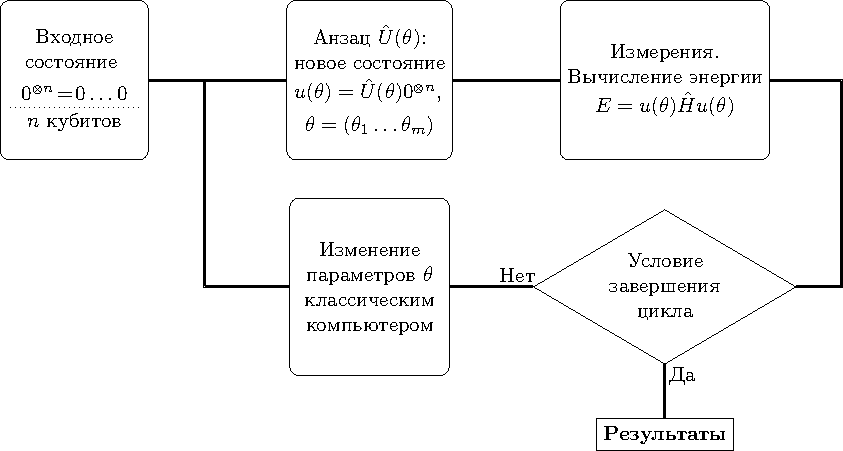
\includegraphics[width=15cm]{figures/scheme_simple.pdf}\\
  \caption{Общая схема квантового вариационного алгоритма. Более подробную схему можно изучить на Рис. \ref{DetailedQuantumVariationAlgorithmScheme}}\label{ShemeVQA}
\end{figure}


\section{Пример, иллюстрирующий особенности алгоритма}


Для иллюстрации алгоритма рассмотрим гамильтониан
\begin{align}\label{H}
\hat{H} = 2\,\hat{\sigma}_{03} + \hat{\sigma}_{30} - 4\,\hat{\sigma}_{11},
\end{align}
который в стандартном базисе $\big\{\ket{00}, \ket{01}, \ket{10}, \ket{11}\!\big\}$ имеет матрицу
\begin{equation}\label{}
H=
\!\!\left(\!
\begin{array}{cccc}
3& 0& 0& \!\!-4 \vphantom{\hat{A}}  \\[2pt]
0& \!\!-1& \!\!-4& 0 \vphantom{\hat{A}}  \\[2pt]
0& \!\!-4& 1& 0 \vphantom{\hat{A}}  \\[2pt]
\!\!-4& 0& 0& \!\!-3 \vphantom{\hat{A}}
\end{array}
\!\!\right).\nonumber
\end{equation}
Используя систему Maple находим собственные значения и собственные состояния в порядке возрастания собственных значений, начиная с основного состояния $\ket{u_0}$ с собственным значением $E_0$:
\begin{align}
E_0&= -5,\; &&\ket{u_0}= \frac{1}{\,\sqrt{5}\,}\,\ket{00}+ \frac{2}{\,\sqrt{5}\,}\,\ket{11}, \label{E0-u0}\\
E_1&= -\sqrt{17},\;\vphantom{\int\limits^A} &&\ket{u_1}= \frac{\sqrt{17}+1}{\,\sqrt{34+2\sqrt{17}\,}\,}\,\ket{01}+ \frac{\sqrt{8}}{\,\sqrt{17+\sqrt{17}\,}\,}\,\ket{10}, \label{E1-u1}\\
E_2&= \sqrt{17},\;\vphantom{\int\limits^A} &&\ket{u_1}= -\frac{\sqrt{17}-1}{\,\sqrt{34-2\sqrt{17}\,}\,}\,\ket{01}+ \frac{\sqrt{8}}{\,\sqrt{17-\sqrt{17}\,}\,}\,\ket{10}, \label{E2-u2}\\
E_3&= 5,\;\vphantom{\int\limits^A} &&\ket{u_3}= -\frac{2}{\,\sqrt{5}\,}\,\ket{00}+ \frac{1}{\,\sqrt{5}\,}\,\ket{11}. \label{E3-u3}
\end{align}
Рассмотрим далее пошаговое выполнение вариационного квантового алгоритма, который позволяет найти состояние, близкое к основному.

\textit{Первый шаг --- выбор анзаца}, т.е. унитарного преобразования $\hat{U}(\bm\theta)$. В гамильтониан~(\ref{H}) не входят операторы вида $\hat{\sigma}_{k2}$ и $\hat{\sigma}_{k2}$ с $k\neq2$, поэтому имеет смысл сразу выбирать анзац так, чтобы при действии на $k\neq2$ он давал вектор состояния с вещественными коэффициентами. Других наводящих соображений относительно формы анзаца не видно, поэтому следует рассмотреть разные варианты. В общем случае вектор параметров $\bm\theta$ четырехмерен. В простейшем варианте анзац с четырехмерным вектором параметров $\bm\theta=(\xi,\lambda,\mu,\nu)$ можно выбирать как композицию экспонент
\begin{equation}\label{ansatz}
\hat{U}(\bm\theta)= \mathrm{e}^{i\xi\hat{\sigma}_{02}}\mathrm{e}^{i\lambda\hat{\sigma}_{03}} \mathrm{e}^{i\mu\hat{\sigma}_{30}} \mathrm{e}^{i\nu\hat{\sigma}_{11}}
\end{equation}
операторов Паули, присутствующих в гамильтониане~(\ref{H}). Вычислим вначале
\begin{multline}\label{}
\mathrm{e}^{i\mu\hat{\sigma}_{30}} \mathrm{e}^{i\nu\hat{\sigma}_{11}}\ket{00}= \big(\cos\:\!\!\mu\,\hat{\sigma}_{00}+ i\sin\:\!\!\mu\,\hat{\sigma}_{30}\big)\big(\cos\:\!\!\nu\ket{00}+ i\sin\:\!\!\nu\ket{11}\big)
\vphantom{\int}\\
=\cos\:\!\!\mu\cos\:\!\!\nu\ket{00}- \sin\:\!\!\mu\sin\:\!\!\nu\ket{11}+ i\sin\:\!\!\mu\cos\:\!\!\nu\ket{00}+ i\cos\:\!\!\mu\sin\:\!\!\nu\ket{11}
\vphantom{\int}\\
=\mathrm{e}^{i\mu}\cos\:\!\!\nu\ket{00}+ i\mathrm{e}^{i\mu}\sin\:\!\!\nu\ket{11}= \mathrm{e}^{i\mu}\cos\:\!\!\nu\ket{00}+ \mathrm{e}^{i(\mu+\pi/2)}\sin\:\!\!\nu\ket{11}.
\nonumber
\end{multline}
Действуя на результат оператором $\mathrm{e}^{i\lambda\hat{\sigma}_{03}}$, получим следующий промежуточный вектор состояния:
\begin{multline}\label{3param}
\mathrm{e}^{i\lambda\hat{\sigma}_{03}} \mathrm{e}^{i\mu\hat{\sigma}_{30}} \mathrm{e}^{i\nu\hat{\sigma}_{11}}\ket{00}= \mathrm{e}^{i\mu}\cos\:\!\!\nu \big(\cos\:\!\!\lambda\,\hat{\sigma}_{00}+ i\sin\:\!\!\lambda\hat{\sigma}_{03}\big)
\ket{00}\\
\qquad\qquad\qquad\qquad\qquad\quad\: +\mathrm{e}^{i(\mu+\pi/2)}\sin\:\!\!\nu \big(\cos\:\!\!\lambda\,\hat{\sigma}_{00}+ i\sin\:\!\!\lambda\hat{\sigma}_{03}\big)
\ket{11} \vphantom{\int}\\
\;\;=\mathrm{e}^{i\mu}\cos\:\!\!\nu
\big(\cos\:\!\!\lambda+ i\sin\:\!\!\lambda\big)\ket{00}+
\mathrm{e}^{i(\mu+\pi/2)}\sin\:\!\!\nu
\big(\cos\:\!\!\lambda+ i\sin\:\!\!\lambda\big)\ket{11}
\vphantom{\int}\\
=\mathrm{e}^{i(\mu+\lambda)}\cos\:\!\!\nu\ket{00}+ \mathrm{e}^{i(\mu+\pi/2-\lambda)}\sin\:\!\!\nu\ket{11}.\quad\,
\end{multline}
Очевидно, что этот анзац не является универсальным.

Варьируя параметры $\lambda,\mu,\nu$, можно получить основное состояние~(\ref{E0-u0}) с точностью до несущественного множителя $\mathrm{e}^{i(\mu+\pi/4)}$, например, при
\begin{equation}\label{param}
\lambda=\pi/4, \quad \mu\in\mathbb{R}, \quad \cos\:\!\!\nu=1/\sqrt{5},
\quad
\sin\:\!\!\nu=2/\sqrt{5}.
\end{equation}
Здесь $\mu$ --- любое, поэтому к нужному результату приводит более простой анзац (при $\mu=0$) $\hat{U}(\bm\theta)= \mathrm{e}^{i\lambda\hat{\sigma}_{03}} \mathrm{e}^{i\nu\hat{\sigma}_{11}}$, однако заранее это нам не известно. Более того основное состояние~(\ref{E0-u0}) можно достигнуть (что заранее также неизвестно и неочевидно) даже однопараметрическим анзацем
\begin{equation*}\label{}
\mathrm{e}^{i\nu\hat{\sigma}_{12}}\ket{00}= \big(\cos\:\!\!\nu\,\hat{\sigma}_{00}+ i\sin\:\!\!\nu\,\hat{\sigma}_{12}\big)\ket{00}= \cos\:\!\!\nu\ket{00}+ \sin\:\!\!\nu\ket{11},
\nonumber
\end{equation*}
с теми же значениями $\cos\:\!\!\nu$ и $\sin\:\!\!\nu$, что и в~(\ref{param}).

Действуя на~(\ref{3param}) оператором $\mathrm{e}^{i\xi\hat{\sigma}_{02}}$, получим вектор состояния
\begin{multline}\label{Phi0}
\ket{\Phi}= \hat{U}(\bm\theta)\ket{00}\;\\
=\big(\cos\:\!\!\xi\,\hat{\sigma}_{00}+ i\sin\:\!\!\xi\,\hat{\sigma}_{02}\big) \big(\mathrm{e}^{i(\mu+\lambda)}\cos\:\!\!\nu\ket{00}+ \mathrm{e}^{i(\mu+\pi/2-\lambda)}\sin\:\!\!\nu\ket{11}\big)\! \vphantom{\int}\\
=\mathrm{e}^{i(\mu+\lambda)}\sin\:\!\!\xi\cos\:\!\!\nu\ket{01}- \mathrm{e}^{i(\mu+\pi/2-\lambda)}\sin\:\!\!\xi\sin\:\!\!\nu\ket{10}
\hspace{6.5em} \vphantom{\int}\\
+\mathrm{e}^{i(\mu+\lambda)}\cos\:\!\!\xi\cos\:\!\!\nu\ket{00}+ \mathrm{e}^{i(\mu+\pi/2-\lambda)}\cos\:\!\!\xi\sin\:\!\!\nu\ket{11},\;\,
\end{multline}
который зависит от четырех параметров. Из формы данного вектора видно, что анзац~(\ref{ansatz}) универсален (с учетом замечания о вещественности коэффициентов, сделанного выше). Основное состояние достигается при произвольном $\mu\in\mathbb{R}$ и
\begin{equation}\label{param1}
\!\!\xi=0, \;\lambda=\!\big\{\pi/4,7\pi/4\big\}, \; \cos\:\!\!\nu=1/\sqrt{5},
\; \sin\:\!\!\nu=\big\{2/\sqrt{5},-2/\sqrt{5}\big\}\\
\end{equation}
или
\begin{equation}\label{param2}
\,\xi=\pi, \;\lambda=\!\big\{\pi/4,7\pi/4\big\}, \; {\cos\:\!\!\nu}=\!-1/\sqrt{5},
\; {\sin\:\!\!\nu}=\big\{\!\!-\:\!\!2/\sqrt{5},2/\sqrt{5}\big\}.
\end{equation}

Для сокращения записи имеет смысл освободиться в~(\ref{Phi0}) от фазового множителя и записать вектор состояния в виде
\begin{multline}\label{Phi}
\ket\Phi= \sin\:\!\!\xi \big(\cos\:\!\!\nu\ket{01}- \mathrm{e}^{i(\pi/2-2\lambda)}\sin\:\!\!\nu\ket{10}\!\big)
\\
+\cos\:\!\!\xi \big(\cos\:\!\!\nu\ket{00}+ \mathrm{e}^{i(\pi/2-2\lambda)}\sin\:\!\!\nu\ket{11}\!\big)
\end{multline}

\textit{Второй шаг --- вычисление энергии состояния}, т.е. среднего значения $\bra\Phi{\hat{H}}\ket\Phi$. Заметим, что первый и второй шаги должны выполняться на квантовых устройствах, а при классической симуляции алгоритма необходимо проводить явные вычисления. Из~(\ref{H}) и~(\ref{Phi}) находим
\begin{multline}\label{}
{\hat{H}}\ket\Phi= \sin\:\!\!\xi\big(2\,\hat{\sigma}_{03}+ \hat{\sigma}_{30}- 4\hat{\sigma}_{11}\big)\! \big(\cos\:\!\!\nu\ket{01}- \mathrm{e}^{i(\pi/2-2\lambda)}\sin\:\!\!\nu\ket{10}\!\big)
\\
+\cos\:\!\!\xi\big(2\,\hat{\sigma}_{03}+ \hat{\sigma}_{30}- 4\hat{\sigma}_{11}\big)\! \big(\cos\:\!\!\nu\ket{00}+ \mathrm{e}^{i(\pi/2-2\lambda)}\sin\:\!\!\nu\ket{11}\!\big)
\hspace{0.2em} \vphantom{\int\limits^A_A}
\\%%%%%%%%%%%%%% |01> |10>
={\sin\:\!\!\xi}\!\left\{\! \big(4\mathrm{e}^{i(\pi/2-2\lambda)}\sin\:\!\!\nu- \cos\:\!\!\nu\big)\ket{01}\right.\hspace{7.6em}
\\
\hspace{16em}\left.-\big(\mathrm{e}^{i(\pi/2-2\lambda)}\sin\:\!\!\nu+ 4\cos\:\!\!\nu\big)\ket{10}\!\right\}
\\%%%%%%%%%%%%%% |00> |11>
+{\cos\:\!\!\xi}\!\left\{\! \big(3\cos\:\!\!\nu-4\mathrm{e}^{i(\pi/2-2\lambda)}\sin\:\!\!\nu\big)\ket{00} \right.\hspace{6.6em}
\\
\left.-\big(4\cos\:\!\!\nu+ 3\mathrm{e}^{i(\pi/2-2\lambda)}\sin\:\!\!\nu\big) \ket{11}\!\right\}\!.\hspace{0.5em}
\nonumber
\end{multline}
Поскольку
\begin{multline}\label{}
\bra\Phi=
\sin\:\!\!\xi \big(\cos\:\!\!\nu\bra{01}- \mathrm{e}^{-i(\pi/2-2\lambda)}\sin\:\!\!\nu\bra{10}\,\big)
\\
+\cos\:\!\!\xi \big(\cos\:\!\!\nu\bra{00}+ \mathrm{e}^{-i(\pi/2-2\lambda)}\sin\:\!\!\nu\bra{11}\,\big),
\hspace{2.2em} \vphantom{\int\limits^A}
\nonumber
\end{multline}
то
\begin{multline}\label{EPhi}
E_{\Phi}= \bra\Phi{\hat{H}}\ket\Phi
\\
=\sin^2\:\!\!\xi\!\left\{\!\cos\:\!\!\nu \big(4\mathrm{e}^{i(\pi/2-2\lambda)}\sin\:\!\!\nu- \cos\:\!\!\nu\big) \right.\hspace{7.6em}
\\
\hspace{16em}\left.+\sin\:\!\!\nu\big(\sin\:\!\!\nu+ 4\mathrm{e}^{-i(\pi/2-2\lambda)}\cos\:\!\!\nu\big)\right\}
\\%%%%%%%%%%%%%% |00> |11>
+\cos^2\:\!\!\xi\!\left\{\!\cos\:\!\!\nu\big(3\cos\:\!\!\nu- 4\mathrm{e}^{i(\pi/2-2\lambda)}\sin\:\!\!\nu\big) \right.\hspace{6.6em}
\\
\hspace{4em}\left.-\sin\:\!\!\nu\big(4\mathrm{e}^{-i(\pi/2-2\lambda)}\cos\:\!\!\nu+ 3\sin\:\!\!\nu\big)\!\right\}
\vphantom{\underbrace{j_|}}
\\
=\sin^2\:\!\!\xi\big(4\sin\:\!\!2\lambda\sin\:\!\!2\nu- \cos\:\!\!2\nu\big)+
\cos^2\:\!\!\xi\big(3\cos\:\!\!2\nu- 4\sin\:\!\!2\lambda\sin\:\!\!2\nu\big).
\vphantom{\widehat{A^|}}
\end{multline}
Разумеется, если взять значения ${\xi,\, \lambda,\, \cos\:\!\!\nu,\, \sin\:\!\!\nu}$ как в~(\ref{param1}) или в~(\ref{param2}), то мы получим энергию основного состояния~(\ref{E0-u0}), т.е.  $E_{\Phi}=-5$.


\textit{Третий шаг --- изменение значений параметров} $\lambda,\mu,\nu$ (с целью минимизации $E_{\Phi}$) и возвращение к первому шагу; предполагается, что в начале выполнения алгоритма начальные значения параметров заданы. Из~(\ref{EPhi}) видно, что на значение $E_{\Phi}$ параметр $\mu$ не влияет, а параметры $\lambda,\nu$ должны варьироваться в области ${[0,\pi]\times[0,\pi]}$. Однако изначально это неизвестно, поэтому все четыре параметра должны варьироваться в области ${[0,2\pi]\times[0,2\pi]\times[0,2\pi]\times[0,2\pi]}$. Имеет смысл установить независимость энергии от параметра $\mu$ (и ее зависимость от остальных параметров) в начале работы алгоритма.

Мы уже знаем, что глобальный минимум энергии достигается для четырех наборов параметров~(\ref{param1}) и~(\ref{param2}). Соответствующие собственные векторы, вычисленные по выражению~(\ref{Phi}) отличаются от~(\ref{E0-u0}) только фазовыми множителями. Теперь необходимо выяснить, имеются ли у функции (трех переменных)~(\ref{EPhi}) другие локальные минимумы.

Используя систему Maple, вычислим производные
\begin{equation*}
\partial_\xi E_{\Phi},\,\; \partial_\lambda E_{\Phi},\,\; \partial_\nu E_{\Phi},\,\;
\end{equation*}
\begin{equation*}
A=\partial_\xi^{\:\!2}E_{\Phi},\,\; B=\partial_\lambda^{\:\!2}E_{\Phi},\,\; C=\partial_\nu^{\:\!2}E_{\Phi},\,\;
\end{equation*}
\begin{equation*}
K= \partial_{\xi\lambda}E_{\Phi},\,\; L=\partial_{\xi\nu}E_{\Phi},\,\; M=\partial_{\lambda\nu}E_{\Phi}.\,\;
\end{equation*}
Находим
\begin{eqnarray*}
\partial_\xi E_{\Phi} &=& 4\sin\:\!\!2\xi\big(2\sin\:\!\!2\lambda\sin\:\!\!2\nu- \cos\:\!\!2\nu\big),
\\
\partial_\lambda E_{\Phi} &=& -8\cos\:\!\!2\xi\cos\:\!\!2\lambda\sin\:\!\!2\nu, \\
\partial_\nu E_{\Phi} &=& \sin^2\:\!\!\xi\big(8\sin\:\!\!2\lambda\cos\:\!\!2\nu+ 2\sin\:\!\!2\nu\big)-
\cos^2\:\!\!\xi\big(6\sin\:\!\!2\nu+ 8\sin\:\!\!2\lambda\cos\:\!\!2\nu\big),
\\
A &=& 8\cos\:\!\!2\xi \big(2\sin\:\!\!2\lambda\sin\:\!\!2\nu-\cos\:\!\!2\nu\big),
\\
B &=& 16\cos\:\!\!2\xi \sin\:\!\!2\lambda \sin\:\!\!2\nu,
\\
C &=& 4\cos^2\:\!\!\xi\big(4\sin\:\!\!2\lambda\sin\:\!\!2\nu- 3\cos\:\!\!2\nu\big) -4\sin^2\:\!\!\xi\big(4\sin\:\!\!2\lambda\sin\:\!\!2\nu- \cos\:\!\!2\nu\big),
\\
K &=& 16\sin\:\!\!2\xi \cos\:\!\!2\lambda \sin\:\!\!2\nu,
\\
L &=& 4\sin\:\!\!2\xi \big(4\sin\:\!\!2\lambda\cos\:\!\!2\nu+ 2\sin\:\!\!2\nu\big),
\\
M &=& -16\cos\:\!\!2\xi \cos\:\!\!2\lambda \cos\:\!\!2\nu.
\end{eqnarray*}
Необходимые и достаточные условия минимума имеют вид
\begin{equation}\label{ExtrConds}
\partial_\xi E_{\Phi}=0,\quad \partial_\lambda E_{\Phi}=0,\quad \partial_\nu E_{\Phi}=0,
\nonumber
\end{equation}
\begin{equation}\label{}
A>0,\qquad
\det\!\left(\!\!
\begin{array}{cc}
A&\!\! K \\
K&\!\! B\vphantom{\hat{A}}
\end{array}
\!\!\!\:\right)\!>0,
\qquad
\det\!\!\!\:\left(\!\!
\begin{array}{ccc}
A&\! K&\! L \\[2pt]
K&\! B&\! M\vphantom{\hat{A}}  \\[2pt]
L&\! M&\! C\vphantom{\hat{A}}
\end{array}
\!\!\right)\!>0.
\nonumber
\end{equation}

Снова проводя вычисления с помощью системы Maple, обнаруживаем четыре точки локального минимума с энергией ${E_\Phi=-\sqrt{17}}$:
\begin{align*}
\xi=\frac{\pi}{2}, &\qquad\lambda=\frac{\pi}{4}, \qquad \nu=\pi-\,\frac{1}{2}\,\arctan(4),\\
\xi=\frac{\pi}{2}, &\qquad\lambda=\frac{\pi}{4}, \qquad\:\! \!\!\:\nu=2\pi-\,\frac{1}{2}\,\arctan(4),\\
\xi=\frac{\pi}{2}, &\qquad\lambda=\frac{3\pi}{4}, \quad\;\, \nu=\frac{1}{2}\,\arctan(4),\\
\xi=\frac{\pi}{2}, &\qquad\lambda=\frac{3\pi}{4}, \quad\;\, \nu=\pi+\,\frac{1}{2}\,\arctan(4).
\end{align*}

Таким образом, в процессе оптимизации целевой функции должны использоваться методы, которые позволяют избежать попадания в точку локального минимума, например, метод отжига.


%#############################################################################################################################################################################################################################
%################################################################### 2 Вариационный квантовый алгоритм на основе метода отжига ###############################################################################################
%#############################################################################################################################################################################################################################

\chapter{Вариационный квантовый алгоритм на основе метода отжига}

%#############################################################################################################################################################################################################################
%##################################################################################### 2.1 Метод отжига ######################################################################################################################
%#############################################################################################################################################################################################################################

\section{Метод отжига}\label{MethAnn}

Метод отжига или, подробнее, метод имитации отжига относится к семейству методов Монте-Карло, разработанных для поиска \textit{глобального}\linebreak минимума целевой функции. Этот метод обладает одним существенным преимуществом по сравнению с аналитическими методами оптимизации: он применим к целевым функциям произвольной природы. Особенно важно то, что метод отжига полностью сохраняет свою эффективность в задачах, где целевая функция не дифференцируема и при этом имеет большое число локальных минимумов. По этой причине, метод отжига, как фундаментальная концепция в теории глобальной оптимизации, широко используется в квантовых вычислениях, особенно в вариационных квантовых алгоритмах (в их квантовой реализации, а не классической эмуляции), где вычисление целевой функции не обладает достаточной точностью. Основная идея метода заключается в постепенном снижении "температуры"\, системы, чтобы достичь состояния с минимальным значением целевой функции (далее, для краткости, энергии). В этом разделе подробно рассматривается классический вариант отжига и детали его практического применения.

Классический метод отжига основывается на аналогии с физическим процессом термического отжига, при котором материал медленно охлаждается, чтобы избежать образования дефектов и достичь состояния минимальной энергии. Математическое обоснование метода связано с распределением Больцмана, которое описывает вероятность состояния системы при заданной температуре $T$ формулой
\begin{equation}
p(x) = \frac{1}{Z(T)} \exp\left(-\frac{E(x)}{k_B T}\right), \nonumber
\end{equation}
в которой $E(x)$ — энергия состояния $x$, $k_B$ — постоянная Больцмана, а $Z(T)$ — статистическая сумма. Процесс отжига является дискретным и моделирует систему, которая на каждом шаге может переходить между состояниями $x$ и $y$ с вероятностью, которая зависит от разности энергий $\Delta E= E(y)-E(x)$:
\begin{equation}\label{prob}
p(x\rightarrow y) = \min\left(1, \exp\left(-\frac{\Delta E}{k_B T}\right)\right).
\end{equation}
С вероятностью $1-p(x\rightarrow y)$ состояние системы не изменяется.

В самом общем случае в абстрактную математическую постановку задачи оптимизации методом отжига входят следующие данные.

\textbf{Список данных}\vspace{-2ex}
\begin{enumerate}
  \item Множество состояний $C$.
  \item Энергия (целевая функция) $E: C\rightarrow\mathbf{R}$.
  \item Семейство $Rnd=\big\{R_s\big\}_{s\in J}$ отображений $R_s\!:C\rightarrow C$, где множество индексов $J$, вообще говоря, не счетно.
  \item Начальная температура $T$, минимальная температура $T_{min}$ и закон ее понижения  $T_k\rightarrow T_{k+1}=F(T_k,k)$, где $k$ --- шаг процесса отжига.
\end{enumerate}

Практическая реализация имитации отжига обычно осуществляется\linebreak посредством последовательности конечного числа шагов --- случайных испытаний. Каждое испытание состоит, во-первых, из случайного выбора некоторого отображения $R_s\in Rnd$, задающего переход $x\rightarrow y=R_s(x)$, т.е. этот переход выбирается случайным образом из некоторого семейства возможностей. В зависимости от типа задачи вероятностное распределение (вероятностная мера) на $Rnd$ выбирается в достаточно широком диапазоне (нормальное распределение, распределение Коши, равномерное распределение и т.д.). Такое распределение, в свою очередь, может зависеть от температуры.

Во-вторых, с помощью генератора псевдослучайных чисел выбирается значение $\varepsilon$ равномерно распределенной на интервале {(0,\;1)} случайной величины. Если выполнено условие
\begin{equation}\label{prob1}
\varepsilon < \exp\:\!\frac{E(x)-E(y)}{k_B T}, \nonumber
\end{equation}
то переход $x \rightarrow y$ принимается даже если энергия нового состояния, $E(y)$, больше, чем энергия $E(x)$ предыдущего состояния. В противном случае, когда $E(y)\leqslant E(x)$, данное условие выполняется. Такой способ перехода предохраняет от попадания в локальный минимум, в особенности, если процедуру отжига повторять несколько раз. Наконец, в третьих, на каждом шаге производится понижение температуры в соответствии с некоторым правилом. Постепенное уменьшение температуры приводит к уменьшению вероятности перехода в состояния с более высокой энергией, в то время как система стремится к состоянию глобального минимума энергии.


\section{Алгоритм}

\noindent
\textbf{Краткое описание алгоритма}

В задачах квантовой оптимизации в системе из $n$ кубитов множество состояний $C$, входящее в \textit{Список данных} из предыдущего раздела~\ref{MethAnn}, является подмножеством в пространстве состояний системы ${\mathcal{H}_n}$. Оно возникает в результате применения параметризованного анзаца ${\hat{U}(\bm\theta)}$ к начальному состоянию ${\ket{0\ldots0}=\ket0^{\!{\scriptscriptstyle\otimes}{n}}}$, так что ${\ket{u(\bm\theta)}= \hat{U}(\bm\theta)\ket0^{\!{\scriptscriptstyle\otimes}{n}}}$, где
\begin{equation*}
\bm\theta= (\theta_1,\ldots,\theta_m)\in\Omega= [0, 2\pi]^m.
\end{equation*}
Таким образом, ${\ket{u(\bm\theta)}}\in C$ --- это функция на пространстве параметров $\Omega$ со значениями в ${\mathcal{H}_n}$; при этом $C$ не является подпространством в ${\mathcal{H}_n}$. Энергия (целевая функция на $\Omega$) из \textit{Списка данных, п.\,2}, определяется выражением $E(\bm\theta)= \bra{u(\bm\theta)}\hat{H}\ket{u(\bm\theta)}$.

В предлагаемом алгоритме выбор отображения из семейства $Rnd$ (\textit{Список данных, п.\,3}) равновероятен в отношении любого отображения в следующем смысле.
С помощью генератора псевдослучайных чисел\linebreak выбирается $m$ значений ${\varepsilon_i\in(0,\;1),\, i=1,\ldots,m}$ случайной величины, равномерно распределенной на данном интервале, а затем формируется случайный вектор
\begin{equation*}
\delta\bm\theta=(\delta\theta_1,\ldots,\delta\theta_m)\in\Omega,\quad \delta\theta_i= \varepsilon_i\pi.
\end{equation*}
Отображение $R_{\delta\bm\theta}\!: C\rightarrow C$ определяется формулой ${\ket{u(\bm\theta)} \mapsto \ket{u(\bm\theta\!+\!\delta\bm\theta)}}$, где вектор ${\bm\theta+\delta\bm\theta}$ берется по модулю $2\pi$. Далее производим понижение\linebreak температуры (\textit{Список данных, п.\,4}) по простейшей схеме равномерного уменьшения ее значения на каждом шаге процесса отжига $T_{k+1}\!=T_k-\tau$, где выбор значения $\tau$ производится на основе численных экспериментов с конкретной задачей.

Краткая формулировка алгоритма на уровне псевдокода выглядит следующим образом.

\noindent
\textbf{Вариационная квантовая оптимизация методом отжига}$\vphantom{\int\limits^a}$

\noindent
1.\; Вводим начальный вектор $\bm\theta\in\Omega$, минимальную температуру ${T_{min}}$,\\
$\hphantom{1.\;}$ текущую температуру ${T\!>\!T_{min}}$ и значение $\tau$. Положим $\bm\theta_0=\bm\theta$.

\noindent
\textcolor{red}{\textbf{2}}.\; Генерируем состояние ${\ket{u(\bm\theta)}}$ и вычисляем энергию $E(\bm\theta)$ при\\
$\hphantom{2.\;}$ текущей температуре $T$.

\noindent
3.\; Генерируем случайный вектор ${\delta\bm\theta\in\Omega}$,\;  ${\bm\theta_1= \bm\theta+ \delta\bm\theta\; (\mathrm{mod}\;2\pi)}$.\\
$\hphantom{3.\;}$ Вычисляем энергию $E(\bm\theta_1)$.

\noindent
4.\; Если ${E(\bm\theta_1)\!\leqslant\!E(\bm\theta)}$, то полагаем ${\bm\theta\!=\!\bm\theta_1}$ и ${\bm\theta_0\!=\!\bm\theta_1}$.
Иначе генерируем\\
$\hphantom{4.\;}$  ${\varepsilon\in(0,1)}$ и если ${\varepsilon<\exp\{[E(\bm\theta)- E(\bm\theta_1)]/T\}}$, то полагаем ${\bm\theta\!=\!\bm\theta_1}$.

\noindent
5.\; Понижаем температуру: ${T \mapsto T-\tau}$.

\noindent
6.\; Если ${T\!>\!T_{min}}$, то переходим к метке \textcolor{red}{\textbf{2}}.\; Иначе выходим с результатом\\
$\hphantom{6.\;}$ ${\ket{u(\bm\theta_0)}}$ и $E(\bm\theta_0)$.

Теперь рассмотрим программную реализацию вариационного квантового алгоритма с оптимизацией методом отжига.

\noindent
\textbf{Полное описание алгоритма. Общая структура программы}

Разработанная программа реализует вариационный квантовый алгоритм с классическим оптимизатором на основе метода имитации отжига (simulated annealing). На вход подаётся гамильтониан в базисе Паули, после чего осуществляется поиск минимума энергии в пространстве параметризованных квантовых состояний, генерируемых вариационным анзацем. Программа построена модульно и позволяет последовательно:

\begin{enumerate}
    \item Прочитать описание гамильтониана из текстового файла;
    \item Построить вариационный анзац в виде произведения экспонент Паули-операторов;
    \item Численно вычислить энергию состояния $E(\bm\theta)$;
    \item Найти минимум энергии методом отжига;
    \item Вывести подробную информацию о найденном состоянии и параметрах анзаца.
\end{enumerate}

\noindent
\textbf{Описание гамильтониана}

Гамильтониан $\hat{H}$ вводится в виде линейной комбинации операторов Паули:

\begin{equation}
    \hat{H} = \sum_{k=1}^K c_k \bigotimes_{j=1}^n \sigma_{k_j}^{(j)}
\end{equation}

где $c_k \in \mathbb{C}$~--- коэффициенты, $\sigma_{k_j} \in \{I, X, Y, Z\}$~--- операторы Паули для $j$-го кубита.

В файле \texttt{hamiltonian\_operators.txt} каждая строка имеет вид:

\begin{center}
\texttt{[действительная часть] [мнимая часть] [строка Паули]}
\end{center}

Например, строка
\begin{lstlisting}[language=Python]
2.0 0.0 03
\end{lstlisting}
задаёт слагаемое $2.0 \cdot \sigma_0 \otimes \sigma_3 = 2I \otimes Z$.

\noindent
\textbf{Загрузка гамильтониана}

Для загрузки и парсинга гамильтониана используется функция:

\begin{lstlisting}[language=Python]
def read_hamiltonian_data(file_path):
    lines = read_file_lines(file_path, ignore_comments=False)
    pauli_operators = []
    pauli_strings = []
    for line in lines:
        parts = line.strip().split()
        if len(parts) == 3:
            real_part, imag_part, index_str = (
                float(parts[0]),
                float(parts[1]),
                str(parts[2]),
            )
            coefficient = np.complex128(real_part + imag_part * 1j)
            index_list = [int(c) for c in index_str]
            if coefficient != 0:
                pauli_operators.append((coefficient, index_list))
            pauli_strings.append(index_list)
    return pauli_operators, pauli_strings
\end{lstlisting}

\noindent
\textbf{Вариационный анзац в базисе Паули}

Анзац реализован в виде произведения операторов Паули, параметризованных углами $\bm\theta$:

\begin{equation}
    \hat{U}(\bm\theta) = \prod_{j=1}^m \exp\Big(i \theta_j \cdot |\!|c_j|\!| \cdot \hat{\sigma}_{K_j}\Big)
\end{equation}

где $\hat{\sigma}_{K_j}$~--- базисные операторы Паули, входящие в гамильтониан, а $c_j$~--- соответствующие коэффициенты.

Для разложения экспоненты используется формула Эйлера:

\begin{equation}
    \exp(i\alpha \hat{\sigma}) = \cos\alpha \cdot I + i\sin\alpha \cdot \hat{\sigma}
\end{equation}

Реализация разложения анзаца по базису Паули:

\begin{lstlisting}[language=Python]
def calculate_ansatz(
    theta: np.ndarray, pauli_operators: List[Tuple[complex, List[int]]]
) -> Tuple[Dict[Tuple[int, ...], complex], str, str]:
    operator_length = len(pauli_operators[0][1])
    result = {tuple([0] * operator_length): 1.0}
    for t, (coeff, op) in zip(theta, pauli_operators):
        angle = t * abs(coeff)
        cos_t = np.cos(angle)
        sin_t = np.sin(angle)
        new_result = {}
        op_tuple = tuple(op)
        for existing_op, existing_coeff in result.items():
            new_result[existing_op] = (
                new_result.get(existing_op, 0) + existing_coeff * cos_t
            )
            compose_coeff, compose_op = pauli_compose(existing_op, op_tuple)
            final_coeff = existing_coeff * 1j * sin_t * compose_coeff
            new_result[compose_op] = new_result.get(compose_op, 0) + final_coeff
        result = new_result
    symbolic_str, numeric_str = format_ansatz(pauli_operators, result)
    return result, symbolic_str, numeric_str
\end{lstlisting}

\noindent
\textbf{Алгебра Паули и композиция операторов}

Композиция двух операторов Паули $\hat{\sigma}_K$, $\hat{\sigma}_L$ реализуется покубитно согласно таблице умножения:

\begin{equation}
    \hat{\sigma}_i \hat{\sigma}_j =
    \begin{cases}
        \hat{\sigma}_0 & \text{если}\;\; i = j \\
        \hat{\sigma}_j & \text{если}\;\; i = 0 \\
        \hat{\sigma}_i & \text{если}\;\; j = 0 \\
        \pm i\hat{\sigma}_k & \text{иначе}
    \end{cases}
\end{equation}
\noindent
где $i,j,k \in \{0,1,2,3\}$, $\hat{\sigma}_0 = I$.

Программная реализация:

\begin{lstlisting}[language=Python]
def multiply_pauli(i: int, j: int) -> Tuple[complex, int]:
    if i == j:
        return (1, 0)
    if i == 0:
        return (1, j)
    if j == 0:
        return (1, i)
    return PAULI_MAP.get((i, j), (1, 0))

def pauli_compose(s1: tuple, s2: tuple) -> Tuple[complex, tuple]:
    coefficient = 1.0
    result = []
    for a, b in zip(s1, s2):
        coeff, idx = multiply_pauli(a, b)
        coefficient *= coeff
        result.append(idx)
    return coefficient, tuple(result)
\end{lstlisting}

\noindent
\textbf{Вычисление энергии состояния}

Энергия состояния для текущего набора параметров $\bm\theta$ вычисляется как математическое ожидание гамильтониана в состоянии $\ket{u(\bm\theta)}$:

\begin{equation}
    E(\bm\theta) = \bra{0} \hat{U}^\dagger(\bm\theta)\, \hat{H} \, \hat{U}(\bm\theta) \ket{0}
\end{equation}

Реализация последовательной композиции операторов $U^\dagger H U$ и вычисления среднего значения:

\begin{lstlisting}[language=Python]
def compute_uhu(
    u_dict: Dict[Tuple[int, ...], complex], h_terms: List[Tuple[complex, List[int]]]
) -> Dict[Tuple[int, ...], complex]:
    uhu_dict = {}
    for coeff_h, op_h in h_terms:
        op_h_tuple = tuple(op_h)
        for j_op, j_coeff in u_dict.items():
            conj_j_coeff = np.conj(j_coeff)
            c1, op_uh = pauli_compose(j_op, op_h_tuple)
            for k_op, k_coeff in u_dict.items():
                c2, op_uhu = pauli_compose(op_uh, k_op)
                total_coeff = conj_j_coeff * k_coeff * coeff_h * c1 * c2
                uhu_dict[op_uhu] = uhu_dict.get(op_uhu, 0) + total_coeff
    return uhu_dict

def calculate_expectation(uhu_dict: Dict[Tuple[int, ...], complex]) -> float:
    expectation = 0.0
    for op, coeff in uhu_dict.items():
        if all(p in (0, 3) for p in op):
            expectation += coeff.real
    return expectation
\end{lstlisting}

Вклад в среднее значение дают только те операторы Паули, которые не изменяют состояние $\ket{0\ldots0}$, то есть состоящие только из $I$ и $Z$ на каждом кубите.

\noindent
\textbf{Метод имитации отжига (Simulated Annealing)}

Поиск глобального минимума осуществляется методом имитации отжига, который повторяет физический процесс медленного охлаждения системы. На каждом шаге генерируется новое состояние $\bm\theta' = \bm\theta + \delta\bm\theta$ с малым случайным возмущением, и принимается по правилу Метрополиса:

\begin{equation}
    P_{\text{accept}} =
    \begin{cases}
        1, & \text{если } E(\bm\theta') < E(\bm\theta) \\
        \exp\left(-\dfrac{E(\bm\theta')-E(\bm\theta)}{T}\right), & \text{иначе}
    \end{cases}
\end{equation}

Температура $T$ постепенно понижается по закону $T_{k+1} = \alpha T_k$, где $0 < \alpha < 1$.

\begin{equation}
    T_{k+1} = \alpha T_k
\end{equation}

Реализация основного цикла отжига:

\begin{lstlisting}[language=Python]
def simulated_annealing(
    initial_theta: np.ndarray,
    pauli_operators: List[Any],
    progress: Any,
    task: Any,
    initial_temp: float = 1000.0,
    cooling_rate: float = 0.99,
    min_temp: float = 1e-5,
    num_iterations_per_temp: int = 500,
    step_size: float = 0.5,
) -> Tuple[np.ndarray, float]:
    current_theta = initial_theta.copy()
    best_theta = current_theta.copy()
    best_energy = float("inf")
    rng = np.random.default_rng()
    temp = initial_temp
    thermalization_steps = int(num_iterations_per_temp * 0.2)
    while temp > min_temp:
        # Термализация
        for _ in range(thermalization_steps):
            neighbor_theta = generate_neighbor_theta(current_theta, step_size)
            ansatz_dict, _, _ = calculate_ansatz(neighbor_theta, pauli_operators)
            uhu_dict = compute_uhu(ansatz_dict, pauli_operators)
            current_energy = calculate_expectation(uhu_dict)
            if current_energy < best_energy:
                best_theta = neighbor_theta.copy()
                best_energy = current_energy
            current_theta = neighbor_theta.copy()
            if progress is not None:
                progress.update(task, advance=1)
        # Основной цикл
        for _ in range(num_iterations_per_temp):
            perturbation = rng.normal(0, step_size * (temp / initial_temp), current_theta.shape)
            neighbor_theta = (current_theta + perturbation) % (2 * np.pi)
            ansatz_dict, _, _ = calculate_ansatz(neighbor_theta, pauli_operators)
            uhu_dict = compute_uhu(ansatz_dict, pauli_operators)
            current_energy = calculate_expectation(uhu_dict)
            energy_diff = current_energy - best_energy
            if energy_diff < 0 or rng.random() < np.exp(-energy_diff / temp):
                current_theta = neighbor_theta.copy()
                if current_energy < best_energy:
                    best_theta = current_theta.copy()
                    best_energy = current_energy
            if progress is not None:
                progress.update(task, advance=1)
        temp *= cooling_rate
    return best_theta, best_energy
\end{lstlisting}

\noindent
\textbf{Визуализация и логирование результата}

Для удобства анализа и отладки программа реализует вывод промежуточных и итоговых результатов в консоль в виде таблиц, панелей и прогресс-баров с помощью библиотеки \texttt{rich}, а также ведёт лог-файл всего вывода. В частности, реализованы функции:

\begin{lstlisting}[language=Python]
def print_hamiltonian(console, pauli_operators): ...
def print_pauli_table(console, pauli_operators): ...
def print_composition_table(console, pauli_compose, pauli_strings): ...
\end{lstlisting}

Итоговое значение энергии и параметры оптимального анзаца выводятся в символьном и численном виде.


\section{Сравнительные результаты тестирования}

Для тестирования алгоритма на системе из четырех кубитов будет использоваться гамильтониан
\begin{multline}\label{OH}
\hat{H}_{\scriptscriptstyle OH} = 0.501\,\hat{\sigma}_{1230} - 0.501\,\hat{\sigma}_{2103} - 1.252\,\hat{\sigma}_{0330} \\
- 1.453\,\hat{\sigma}_{2323} + 1.700\,\hat{\sigma}_{1010} + 0.223\,\hat{\sigma}_{1313},\quad
\end{multline}
взятый из работы~\cite{Cawley2013}, в которой изучается спектроскопия основного состояния гидроксильной группы $\mathrm{OH}^-$; гамильтониан переписан в базисе Паули и редуцирован по нулевому уровню энергии (т.е. учтена только бесследовая часть оператора). Сравнительное тестирование включает в себя две задачи: во-первых, сравнительное тестирование двух методов Монте-Карло выбора нового набора параметров, а именно, метода отжига и метода случайного поиска; во-вторых, сравнительное тестирование анзацев --- универсального анзаца, построенного на основе базисных операторов Паули из $\hat{H}_{\scriptscriptstyle OH}$, и нескольких "угаданных"\, пробных анзацев.


Универсальный анзац имеет вид
\begin{equation}\label{ansatz-OH}
\hat{U}(\bm\theta)= \mathrm{e}^{i\theta_4\hat{\sigma}_{0330}} \mathrm{e}^{i\theta_3\hat{\sigma}_{1313}} \mathrm{e}^{i\theta_2\hat{\sigma}_{2103}} \mathrm{e}^{i\theta_1\hat{\sigma}_{1230}},
\end{equation}
где $\theta_k\in[0,2\pi),\; k=1,2,3,4$. Он записан на основе операторов Паули из гамильтониана~(\ref{OH}) за исключением операторов $\hat{\sigma}_{1100}$   $\hat{\sigma}_{2323}$, которые дублируются оператором $\hat{\sigma}_{1313}$. Последний выбран только потому, что он входит в гамильтониан с минимальным коэффициентом.

\noindent
\textbf{Сравнительный анализ параметров отжига}

Для оценки эффективности вариационного квантового алгоритма с оптимизацией методом имитационного отжига были проведены серии тестов с различными наборами параметров отжига. В качестве эталонного значения использовалась энергия основного состояния, равная $-3.601$. В каждом тесте варьировались следующие параметры: начальная температура (\texttt{initial\_temp}), множитель охлаждения (\texttt{cooling\_rate}), минимальная температура (\texttt{min\_temp}), число итераций на каждой температуре (\texttt{num\_iterations\_per\_temp}), а также стандартное отклонение для шума параметров $\theta$ (\texttt{step\_size}).

Полученные результаты позволяют выделить основные закономерности:

\begin{itemize}
    \item При фиксированных начальной температуре и числе итераций на температуре уменьшение шага $step\_size$ приводит к ухудшению результата: алгоритм хуже исследует пространство параметров и чаще застревает в локальных минимумах. Наилучшие значения энергии наблюдались при $step\_size = 0.1$.
    \item Увеличение числа итераций на каждой температуре не приводит к принципиальному улучшению результата, хотя небольшое положительное влияние имеет место.
    \item Повышение начальной температуры (например, до 1000) также не даёт существенного выигрыша, указывая на то, что роль этого параметра в пределах выбранных диапазонов невелика.
    \item Во всех тестах достигнутое значение энергии оставалось выше эталонного примерно на $0.20-0.24$ единицы, что может быть связано с ограничениями самого метода или особенностями выбора анзаца.
\end{itemize}

Таким образом, можно сделать вывод, что параметры $step\_size$ и $num\_iterations\_per\_temp$ оказывают наибольшее влияние на итоговую энергию, однако даже при их оптимизации достичь эталонного значения не удалось. Это свидетельствует о необходимости дальнейшей доработки схемы оптимизации: возможно, стоит рассмотреть более сложные схемы охлаждения, адаптивное изменение шага или комбинированные алгоритмы поиска. Полученные результаты подчеркивают важность тонкой настройки параметров имитационного отжига для задач вариационной квантовой оптимизации.



%#########################################################################################################################################################################################################################
%################################################################################################### Заключение ##########################################################################################################
%#########################################################################################################################################################################################################################

\addcontentsline{toc}{chapter}{\hspace{5.5mm} Заключение}
\chapter*{Заключение}

В работе получены следующие основные результаты:
\begin{enumerate}
    \item{Изучены теоретические основы вариационных квантовых алгоритмов, включая формализм базиса Паули и построение анзаца для многокубитных систем.}
    \item{Реализован и протестирован алгоритм вариационной квантовой оптимизации с использованием метода имитации отжига для поиска глобального минимума энергии гамильтониана.}
    \item{Проведён сравнительный анализ эффективности различных параметров отжига и показано влияние выбора анзаца и схемы оптимизации на точность и сходимость алгоритма.}
    \item{Разработана и описана программная реализация алгоритма на языке Python, позволяющая на практике моделировать процесс вариационной оптимизации для квантовых систем.}
\end{enumerate}



%#########################################################################################################################################################################################################################
%################################################################################################### Литература ##########################################################################################################
%#########################################################################################################################################################################################################################

\addcontentsline{toc}{chapter}{\hspace{5.5mm} Литература}
\begin{thebibliography}{99}
    \bibitem{Tsirulev2020}
    V. V. Nikonov, A. N. Tsirulev. \textit{Pauli basis formalism in quantum computations}. Volume 8, No 3, pp. 1 – 14, 2020.\\
    (\href{https:doi.org/10.26456/mmg/2020-831} {\textit{doi:10.26456/mmg/2020-831}})

    \bibitem{Preskill2018}
    J. Preskill. \textit{Quantum Computing in the NISQ era and beyond}. Quantum, vol. 2, p. 79, 2018.\\
    (\href{https://quantum-journal.org/papers/q-2018-08-06-79/}{\textit{quantum-journal:q-2018-08-06-79}})

    \bibitem{Cerezo2021}
    M. Cerezo, et al. \textit{Variational Quantum Algorithms}. Nature Reviews Physics, vol. 3, pp. 625-644, 2021.\\
    (\href{https://www.nature.com/articles/s42254-021-00348-9}{\textit{nature:42254-021-00348-9}})

    \bibitem{Peruzzo2014}
    A. Peruzzo, et al. \textit{A variational eigenvalue solver on a photonic quantum processor}. Nature Communications, vol. 5, p. 4213, 2014.\\
    (\href{https://www.nature.com/articles/ncomms5213}{\textit{nature:ncomms5213}})

    \bibitem{Farhi2014}
    E. Farhi, J. Goldstone, and S. Gutmann. \textit{A Quantum Approximate Optimization Algorithm}. arXiv preprint arXiv:1411.4028, 2014.\\
    (\href{https://arxiv.org/abs/1411.4028}{\textit{arXiv:1411.4028}})

    \bibitem{Cawley2013}\label{Cawley2013}
    N. Cawley, Z. Howard, M. Kleinert et al. \textit{Analytical study of level crossings in the Stark-Zeeman spectrum of ground state OH}. Eur. Phys. J. D, vol. 67, 233, 2013.\;--\; M. Bhattacharya. S. Marin, M. Kleinert. \textit{Coherent cancellation of geometric phase for the OH molecule in external fields}, 2014.
    (\url{https://doi.org/10.48550/arXiv.1404.6285})

    \bibitem{Kandala2017}
    A. Kandala, et al. \textit{Hardware-efficient variational quantum eigensolver for small molecules and quantum magnets}. Nature, vol. 549, pp. 242-246, 2017.\;    (\href{https://www.nature.com/articles/nature23879}{\textit{nature:nature23879}})

    \bibitem{Harrow2009}
    A. W. Harrow, A. Hassidim, and S. Lloyd. \textit{Quantum algorithm for linear systems of equations}. Physical Review Letters, vol. 103, no. 15, p. 150502, 2009.\\
    (\href{https://journals.aps.org/prl/abstract/10.1103/PhysRevLett.103.150502}{\textit{aps:PhysRevLett.103.150502}})

    \bibitem{Biamonte2017}
    J. Biamonte, et al. \textit{Quantum machine learning}. Nature, vol. 549, pp. 195-202, 2017.\\
    (\href{https://www.nature.com/articles/nature23474}{\textit{nature:nature23474}})

    \bibitem{Lopatin}
    A. A. Lopatin. \textit{Квантовая механика и её приложения}. Санкт-Петербургский Государственный Университет.\\
    (\href{https://math.spbu.ru/user/gran/sb1/lopatin.pdf}{\textit{math.spbu:user/gran/sb1/lopatin}})

    \bibitem{Aspuru-Guzik2005}
    A. Aspuru-Guzik, A. D. Dutoi, P. J. Love, M. Head-Gordon. \textit{Simulated Quantum Computation of Molecular Energies}. Science, vol. 309, no. 5741, pp. 1704-1707, 2005.\\
    (\href{https://www.science.org/doi/10.1126/science.1113479}{\textit{science:1113479}})

    \bibitem{Schuld2015}
    M. Schuld, I. Sinayskiy, F. Petruccione. \textit{An introduction to quantum machine learning}. Contemporary Physics, vol. 56, no. 2, pp. 172-185, 2015.\\
    (\href{https://www.tandfonline.com/doi/abs/10.1080/00107514.2014.964942}{\textit{tandfonline:00107514.2014.964942}})

    \bibitem{Daskin2014}
    A. Daskin, S. Kais. \textit{Decomposition of unitary matrices for finding quantum circuits: Application to molecular Hamiltonians}. The Journal of Chemical Physics, vol. 141, no. 23, p. 234115, 2014.\\
    (\href{https://aip.scitation.org/doi/10.1063/1.4904315}{\textit{aip:1.4904315}})

    \bibitem{Romero2018}
    J. Romero, R. Babbush, J. R. McClean, C. Hempel, P. J. Love, A. Aspuru-Guzik. \textit{Strategies for quantum computing molecular energies using the unitary coupled cluster ansatz}. Quantum Science and Technology, vol. 4, no. 1, p. 014008, 2018.\\
    (\href{https://iopscience.iop.org/article/10.1088/2058-9565/aad3e4}{\textit{iopscience:2058-9565/aad3e4}})

    \bibitem{Havlicek2019}
    V. Havlicek, A. D. Córcoles, K. Temme, A. W. Harrow, A. Kandala, J. M. Chow, J. M. Gambetta. \textit{Supervised learning with quantum-enhanced feature spaces}. Nature, vol. 567, pp. 209-212, 2019.\\
    (\href{https://www.nature.com/articles/s41586-019-0980-2}{\textit{nature:s41586-019-0980-2}})

    \bibitem{Moll2018}
    N. Moll, P. Barkoutsos, L. Bishop, J. M. Chow, A. Cross, D. J. Egger, S. Filipp, A. Fuhrer, J. M. Gambetta, M. Ganzhorn, et al. \textit{Quantum optimization using variational algorithms on near-term quantum devices}. Quantum Science and Technology, vol. 3, no. 3, p. 030503, 2018.\\
    (\href{https://iopscience.iop.org/article/10.1088/2058-9565/aab822}{\textit{iopscience:2058-9565/aab822}})
\end{thebibliography}

%#########################################################################################################################################################################################################################
%################################################################################################### Приложение ##########################################################################################################
%#########################################################################################################################################################################################################################

\addcontentsline{toc}{chapter}{Приложения}
\chapter*{Приложения}
\section*{Приложение А}
\begin{figure}[ht]
\centering
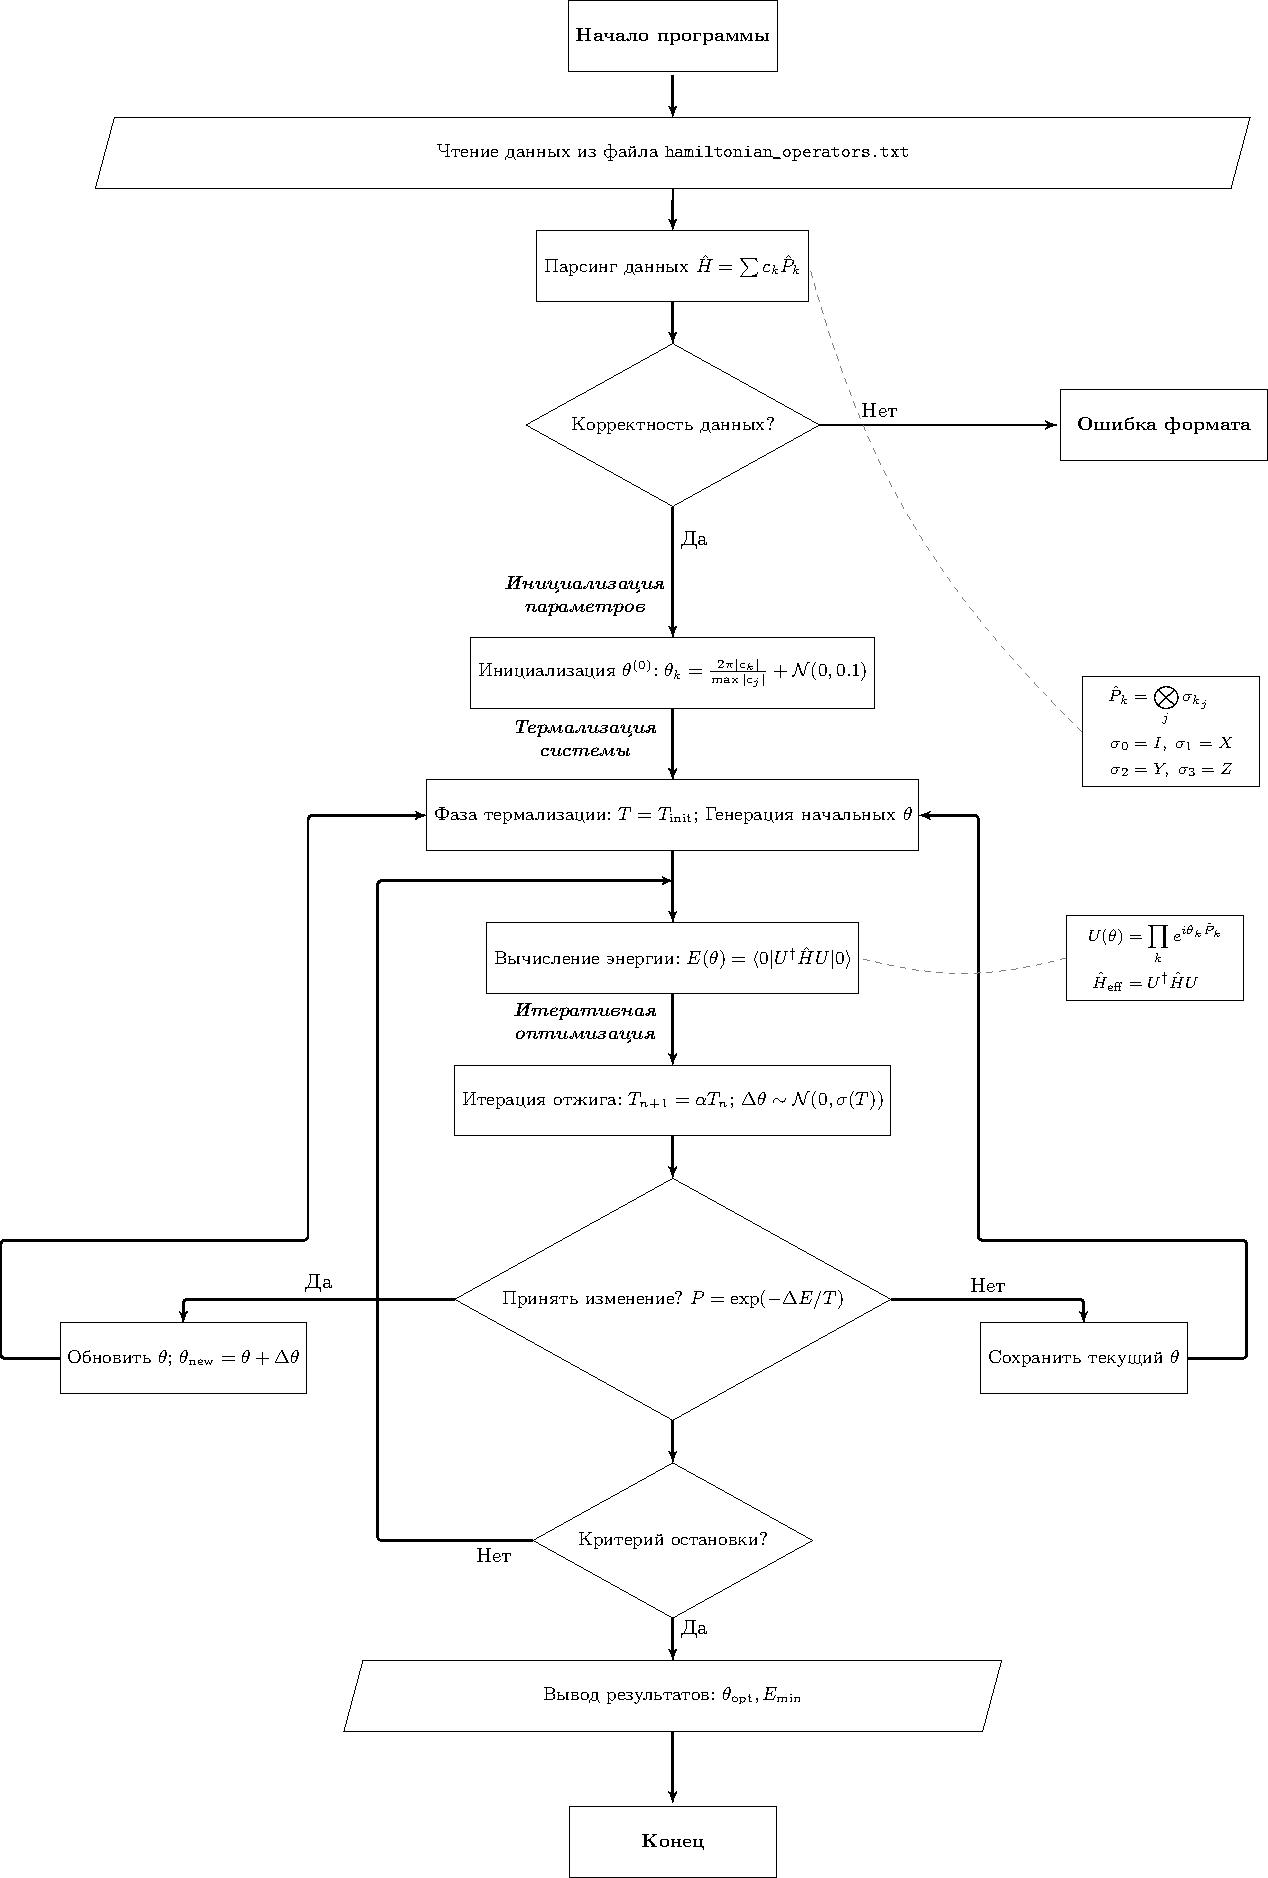
\includegraphics[width=0.6\textwidth]{figures/scheme.pdf}
\caption{Подробная схема квантового вариационного алгоритма}
\label{DetailedQuantumVariationAlgorithmScheme}
\end{figure}
\section*{Приложение Python}
\begin{lstlisting}
import sys
import io
import numpy as np
from pathlib import Path
from rich.console import Console
from rich.table import Table
from rich.panel import Panel
from rich.progress import Progress, BarColumn, TextColumn, SpinnerColumn
from rich import box
from sympy import re as sp_re, im as sp_im
from functools import lru_cache
from typing import Any, List, Dict, Tuple, Union, Callable


def get_base_path() -> Path:
    """
    Определяет базовую директорию проекта.

    Returns:
        Path: Абсолютный путь к папке с .exe-файлом (если приложение заморожено)
              или к корню проекта (в режиме разработки).

    Примечания:
        - sys.frozen (атрибут пакета PyInstaller) используется для определения,
          был ли код скомпилирован в исполняемый файл.
        - Это позволяет корректно определять относительные пути при запуске
          как из исходников, так и из собранного .exe.
    """
    if getattr(sys, "frozen", False):
        # Для скомпилированного EXE возвращаем директорию исполняемого файла.
        return Path(sys.argv[0]).parent
    else:
        # Для разработки возвращаем корень проекта (на уровень выше constants/).
        return Path(__file__).parent.parent


# Абсолютный путь к файлу с гамильтонианом (описание операторов Паули и их коэффициентов).
HAMILTONIAN_FILE_PATH: Path = get_base_path() / "params" / "hamiltonian_operators.txt"

# Абсолютный путь к файлу для логирования вывода (очищается при запуске).
OUTPUT_FILE_PATH: Path = get_base_path() / "output.log"
# Карта произведения для базисных операторов Паули:
# (i, j) -> (мнимая единица с правильным знаком, индекс результата)
# Индексы: 0=I, 1=X, 2=Y, 3=Z
PAULI_MAP = {
    (1, 2): (1j, 3),  # X*Y = iZ
    (2, 1): (-1j, 3),  # Y*X = -iZ
    (3, 1): (1j, 2),  # Z*X = iY
    (1, 3): (-1j, 2),  # X*Z = -iY
    (2, 3): (1j, 1),  # Y*Z = iX
    (3, 2): (-1j, 1),  # Z*Y = -iX
}


def calculate_temp_steps(
    initial_temp: float, cooling_rate: float, min_temp: float
) -> int:
    """
    Вычисляет количество температурных шагов для метода отжига.

    Алгоритм: на каждом шаге температура уменьшается по формуле:
        T_{n+1} = T_n * cooling_rate
    Шаги считаются, пока температура не станет меньше min_temp.

    Args:
        initial_temp (float): Начальная температура.
        cooling_rate (float): Множитель охлаждения (0 < cooling_rate < 1).
        min_temp (float): Минимально допустимая температура.

    Returns:
        int: Число температурных шагов до достижения min_temp.
    """
    steps = 0
    current_temp = initial_temp
    while current_temp > min_temp:
        current_temp *= cooling_rate
        steps += 1
    return steps


def console_and_print(console: Console, message: Any) -> None:
    """
    Выводит сообщение в консоль и дублирует его в лог-файл.

    Args:
        console (Console): объект rich.Console для форматированного вывода.
        message (Any): строка, rich.Panel или другой объект, печатаемый в консоль.

    Примечания:
        - Используется rich для красивого форматирования в консоли и логах.
        - Лог хранит весь вывод, включая цветовые коды (если export_text это поддерживает).
    """
    console.print(message)
    with open(OUTPUT_FILE_PATH, "a", encoding="utf-8") as file:
        file.write(console.export_text() + "\n")


def create_table(
    columns: List[Dict[str, str]],
    data: List[List[Any]],
    title: str,
    border_style: str = "yellow",
) -> Panel:
    """
    Создает таблицу rich.Table и оборачивает ее в rich.Panel для консольного вывода.

    Args:
        columns (List[Dict[str, str]]): Описание столбцов (ключи: name, style, justify).
        data (List[List[Any]]): Массив данных для строк таблицы.
        title (str): Заголовок панели.
        border_style (str): Цвет рамки панели.

    Returns:
        Panel: Панель с таблицей для печати в консоль.
    """
    table = Table(box=box.ROUNDED, border_style=border_style)
    for col in columns:
        table.add_column(
            col["name"],
            justify=col.get("justify", "default"),
            style=col.get("style", ""),
        )
    for row in data:
        table.add_row(*row)
    return Panel(table, title=title, border_style=border_style)


def format_ansatz(
    pauli_operators: List[Tuple[complex, List[int]]],
    result: Dict[Tuple[int, ...], complex],
) -> Tuple[str, str]:
    """
    Форматирует вариационный анзац в символьное и численное представление.

    Args:
        pauli_operators (List[Tuple[complex, List[int]]]): Список операторов Паули для анзаца,
            где каждый оператор представлен кортежем из коэффициента и вектора индексов.
        result (Dict[Tuple[int, ...], complex]): Разложение анзаца после экспоненцирования
            по базису Паули (ключ: вектор индексов, значение: коэффициент).

    Returns:
        Tuple[str, str]: Строки символьного (произведение экспонент) и численного (разложение) представления.

    Символьное представление важно для понимания структуры унитарного оператора:
        $\textcolor{string}{U(\theta) = \exp(i \cdot \theta_1 \cdot c_1 \cdot \sigma_1) \cdot \exp(i \cdot \theta_2 \cdot c_2 \cdot \sigma_2) \cdot \cdots}$

    Численное разложение полезно для анализа конечного состояния оператора:
        $\textcolor{string}{U=\alpha_0\cdot I + \alpha_1\cdot\sigma_1 + \alpha_2\cdot\sigma_2 + \cdots}$
    """
    ansatz_symbolic = "U(θ) = " + " * ".join(
        [
            f"exp(i·θ_{i+1}·{format_complex_number(coeff)}·
            σ_{''.join(map(str, op))})"
            for i, (coeff, op) in enumerate(pauli_operators)
        ]
    )
    ansatz_numeric = "U = " + " + ".join(
        [
            f"{format_complex_number(c)}·σ_{''.join(map(str, op))}"
            for op, c in result.items()
            if abs(c) > 1e-12
        ]
    )
    return ansatz_symbolic, ansatz_numeric


def format_complex_number(c) -> str:
    """
    Форматирует комплексное число (или выражение SymPy) в строку с подавлением артефактов.

    Args:
        c (complex|sympy.Expr): Комплексное число или выражение.

    Returns:
        str: Отформатированное комплексное число (пример: '1.2-3i').

    Особенности:
        - Если число очень близко к нулю (<1e-12), оно не выводится.
        - Мнимая часть ±1 форматируется как ±i.
        - Корректно обрабатывает как стандартные числа, так и объекты SymPy.
    """
    real = float(sp_re(c))
    imag = float(sp_im(c))

    real_str = format_number(real) if abs(real) > 1e-12 else ""
    imag_str = ""

    if abs(imag) > 1e-12:
        abs_imag = abs(imag)
        imag_value = format_number(abs_imag)
        if imag_value == "1":
            imag_str = "i" if imag > 0 else "-i"
        else:
            imag_sign = "" if imag > 0 else "-"
            imag_str = f"{imag_sign}{imag_value}i"

    parts = []
    if real_str:
        parts.append(real_str)
    if imag_str:
        parts.append(imag_str)

    if not parts:
        return "0"

    result = parts[0]
    for part in parts[1:]:
        if part.startswith("-"):
            result += f"-{part[1:]}"
        else:
            result += f"+{part}"

    return result.replace("+ -", "- ").replace("1i", "i").replace(".0i", "i")


def format_number(num: float | int) -> str:
    """
    Форматирует число для вывода, корректно подавляя артефакты округления.

    Args:
        num (float|int): Число для форматирования.

    Returns:
        str: Число в виде строки, без лишних нулей и ошибок округления.
    """
    if abs(num - round(num)) < 1e-15:
        return str(int(round(num)))
    s = f"{num:.14f}".rstrip("0").rstrip(".")
    if s.startswith("."):
        s = "0" + s
    elif s.startswith("-."):
        s = s.replace("-.", "-0.")
    if "." in s:
        int_part, dec_part = s.split(".")
        dec_part = dec_part[:4].ljust(4, "0").rstrip("0")
        s = f"{int_part}.{dec_part}" if dec_part else int_part
    return s


def get_operator_for_console(c: Union[complex, float, int], i: str) -> str:
    """
    Формирует строку для красивого вывода оператора Паули.

    Args:
        c (complex|float|int): Коэффициент перед оператором.
        i (str): Индексная строка оператора (например, '03' для $\textcolor{string}{I\otimes Z}$).

    Returns:
        str: Строка вида '$\textcolor{string}{\sigma_i}$' или '$\textcolor{string}{c\cdot\sigma_i}$'
        (если коэффициент не равен 1).
    """
    if c == 1:
        return f"σ_{i}"
    else:
        return f"{format_complex_number(c)}*σ_{i}"


def initialize_environment() -> Console:
    """
    Инициализирует окружение для запуска программы:
    - Очищает лог-файл с прошлых запусков.
    - Возвращает объект rich.Console для форматированного вывода.

    Returns:
        Console: Готовый к использованию rich.Console.
    """
    if OUTPUT_FILE_PATH.exists():
        OUTPUT_FILE_PATH.unlink()
    return Console(force_terminal=True, color_system="truecolor", record=True)


def print_composition_table(
    console: Console,
    pauli_compose: Callable[[tuple, tuple], Tuple[complex, tuple]],
    pauli_strings: List[List[int]],
) -> None:
    """
    Выводит таблицу композиции операторов Паули для всех их пар.

    Args:
        console (Console): Объект rich.Console.
        pauli_compose (Callable): Функция для композиции двух операторов Паули.
        pauli_strings (List[List[int]]): Список векторных индексов операторов Паули.
    """
    results = []
    # Перебор всех пар операторов Паули
    for s1 in pauli_strings:
        for s2 in pauli_strings:
            coeff, product = pauli_compose(tuple(s1), tuple(s2))
            results.append((s1, s2, format_complex_number(coeff), product))

    table_data = [
        [str(s1), str(s2), str(h).lower(), str(p)] for s1, s2, h, p in results
    ]
    console_and_print(
        console,
        create_table(
            columns=[
                {"name": "Оператор 1", "style": "cyan", "justify": "center"},
                {"name": "Оператор 2", "style": "magenta", "justify": "center"},
                {"name": "Коэффициент", "style": "green", "justify": "center"},
                {"name": "Результат", "style": "red", "justify": "center"},
            ],
            data=table_data,
            title="Композиции операторов Паули",
            border_style="green",
        ),
    )


def print_hamiltonian(
    console: Console, pauli_operators: List[Tuple[complex, List[int]]]
) -> None:
    """
    Выводит гамильтониан в удобочитаемом виде.

    Args:
        console (Console): rich.Console для вывода.
        pauli_operators (List[Tuple[complex, List[int]]]): Список операторов Паули с коэффициентами.
    """
    hamiltonian_str = "H = " + " + ".join(
        [get_operator_for_console(c, "".join(map(str, i))) for c, i in pauli_operators]
    )
    console_and_print(
        console,
        Panel(
            hamiltonian_str,
            title="[bold]Введенный гамильтониан[/bold]",
            border_style="green",
        ),
    )


def print_pauli_table(
    console: Console, pauli_operators: List[Tuple[complex, List[int]]]
) -> None:
    """
    Выводит таблицу всех операторов Паули из гамильтониана.

    Args:
        console (Console): rich.Console для вывода.
        pauli_operators (List[Tuple[complex, List[int]]]): Список операторов Паули с коэффициентами.
    """
    table_data = [[format_complex_number(c), str(i)] for c, i in pauli_operators]
    console_and_print(
        console,
        create_table(
            columns=[
                {"name": "Коэффициент", "style": "cyan"},
                {"name": "Индекс", "style": "magenta", "justify": "center"},
            ],
            data=table_data,
            title="Операторы Паули",
            border_style="purple",
        ),
    )


from pathlib import Path
from typing import List, Union


def read_file_lines(file_path: Union[str, Path], ignore_comments: bool) -> List[str]:
    """
    Считывает строки из файла, игнорируя комментарии (начинающиеся с '#').

    Args:
        file_path (str|Path): Путь к файлу.
        ignore_comments (bool): Если True, строки, начинающиеся с '#', игнорируются.

    Returns:
        List[str]: Список строк без лишних пробелов и пустых строк.

    Raises:
        FileNotFoundError: Если файл не существует.
    """
    file_path = Path(file_path) if not isinstance(file_path, Path) else file_path
    if not file_path.exists():
        raise FileNotFoundError(f"Файл {file_path} не найден.")
    with open(file_path, "r") as file:
        return [
            line.strip()
            for line in file
            if not (ignore_comments and line.strip().startswith("#"))
        ]


def read_hamiltonian_data(
    file_path,
) -> Tuple[List[Tuple[complex, List[int]]], List[List[int]]]:
    """
    Читает список операторов Паули из текстового файла.

    Формат файла:
        <действительная часть> <мнимая часть> <строка Паули>

    Returns:
        Tuple[List[Tuple[complex, List[int]]], List[List[int]]]:
            - Список операторов (коэффициент, индексы Паули)
            - Список только индексов (без коэффициентов)
    """
    lines = read_file_lines(file_path, ignore_comments=False)
    pauli_operators: List[Tuple[complex, List[int]]] = []
    pauli_strings: List[List[int]] = []
    for line in lines:
        parts = line.strip().split()
        if len(parts) == 3:
            real_part, imag_part, index_str = (
                float(parts[0]),
                float(parts[1]),
                str(parts[2]),
            )
            coefficient = np.complex128(real_part + imag_part * 1j)
            index_list = [int(c) for c in index_str]
            if coefficient != 0:
                pauli_operators.append((coefficient, index_list))
            pauli_strings.append(index_list)
    return pauli_operators, pauli_strings


def calculate_ansatz(
    theta: np.ndarray, pauli_operators: List[Tuple[complex, List[int]]]
) -> Tuple[Dict[Tuple[int, ...], complex], str, str]:
    """
    Вычисляет вариационный анзац в виде произведения экспонент операторов Паули.

    Args:
        theta (np.ndarray): Вектор параметров (обычно одного размера с числом операторов).
        pauli_operators (List[Tuple[complex, List[int]]]): Операторы Паули с коэффициентами.

    Returns:
        Tuple[
            Dict[Tuple[int, ...], complex],   # Разложение анзаца по Паули-операторам
            str,                             # Символьное представление (произведение экспонент)
            str                              # Численное разложение
        ]

    Алгоритм:
        $\textcolor{string}{U(\theta) = prod_j exp(i \cdot \theta_j \cdot |c_j| \cdot \sigma_j)}$
        Реализуется по принципу покомпонентного разложения через формулу Эйлера:
            $\textcolor{string}{exp(i\cdot\alpha\cdot\sigma) = cos(\alpha)\cdot I + i\cdot sin(\alpha)\cdot\sigma}$
        С каждым новым оператором результат рекурсивно обновляется через pauli_compose.
    """
    operator_length = len(pauli_operators[0][1])
    result: Dict[Tuple[int, ...], complex] = {tuple([0] * operator_length): 1.0}

    for t, (coeff, op) in zip(theta, pauli_operators):
        angle = t * abs(coeff)  # Используем абсолютное значение коэффициента!
        cos_t = np.cos(angle)
        sin_t = np.sin(angle)
        new_result: Dict[Tuple[int, ...], complex] = {}
        op_tuple = tuple(op)
        for existing_op, existing_coeff in result.items():
            # cos(angle) * I (сохраняем индекс базисного оператора)
            new_result[existing_op] = (
                new_result.get(existing_op, 0) + existing_coeff * cos_t
            )
            # i*sin(angle)*σ (композиция Паули)
            compose_coeff, compose_op = pauli_compose(existing_op, op_tuple)
            final_coeff = existing_coeff * 1j * sin_t * compose_coeff
            new_result[compose_op] = new_result.get(compose_op, 0) + final_coeff
        result = new_result

    symbolic_str, numeric_str = format_ansatz(pauli_operators, result)
    return result, symbolic_str, numeric_str


from typing import Tuple, Dict


def calculate_expectation(uhu_dict: Dict[Tuple[int, ...], complex]) -> float:
    """
    Вычисляет среднее значение энергии $\textcolor{string}{\langle 0 | U^\dagger H U | 0 \rangle для состояния |0 \cdots 0\rangle}$.

    Args:
        uhu_dict (Dict[Tuple[int, ...], complex]): Разложение оператора $\textcolor{string}{U^\dagger HU}$
            по базису Паули (ключ: индекс, значение: коэффициент).

    Returns:
        float: Ожидаемое значение (энергия).

    Примечание:
        - Только те операторы, которые не изменяют $\textcolor{string}{|0 \cdots 0\rangle}$
          (то есть содержащие только I и Z),
          могут дать нетривиальный вклад в среднее значение.
    """
    expectation = 0.0
    for op, coeff in uhu_dict.items():
        if all(p in (0, 3) for p in op):  # Только I или Z на каждом кубите
            expectation += coeff.real
    return expectation


def compute_uhu(
    u_dict: Dict[Tuple[int, ...], complex], h_terms: List[Tuple[complex, List[int]]]
) -> Dict[Tuple[int, ...], complex]:
    """
    Вычисляет оператор $\textcolor{string}{U^\dagger HU}$ $\textcolor{string}{\text{в базисе Паули}}$.

    Args:
        u_dict (Dict[Tuple[int, ...], complex]): Разложение оператора U.
        h_terms (List[Tuple[complex, List[int]]]): Операторы гамильтониана с коэффициентами.

    Returns:
        Dict[Tuple[int, ...], complex]: Разложение $\textcolor{string}{U^\dagger HU}$
          по Паули операторам.

    Алгоритм:
        ($\textcolor{string}{U^\dagger HU}$)_{kl} = sum_{i,j} conj(U_{ik}) * H_{ij} * U_{jl}
        Реализовано через перебор всех Паули-операторов.
    """
    uhu_dict: Dict[Tuple[int, ...], complex] = {}
    u_items = list(u_dict.items())
    for coeff_h, op_h in h_terms:
        op_h_tuple = tuple(op_h)
        for j_op, j_coeff in u_items:
            conj_j_coeff = np.conj(j_coeff)
            c1, op_uh = pauli_compose(j_op, op_h_tuple)
            for k_op, k_coeff in u_items:
                c2, op_uhu = pauli_compose(op_uh, k_op)
                total_coeff = conj_j_coeff * k_coeff * coeff_h * c1 * c2
                uhu_dict[op_uhu] = uhu_dict.get(op_uhu, 0) + total_coeff
    return uhu_dict


def generate_neighbor_theta(
    current_theta: np.ndarray, step_size: float = 0.1
) -> np.ndarray:
    """
    Генерирует новое состояние θ, добавляя нормальный шум
    с заданной дисперсией, и приводит все значения к диапазону [0, 2π).

    Args:
        current_theta (np.ndarray): Текущий вектор параметров.
        step_size (float): Стандартное отклонение для гауссового шума.

    Returns:
        np.ndarray: Новый вектор параметров.
    """
    perturbation = np.random.normal(scale=step_size, size=current_theta.shape)
    return (current_theta + perturbation) % (2 * np.pi)


def generate_shifted_theta(
    pauli_operators: List[Tuple[complex, List[int]]]
) -> np.ndarray:
    """
    Генерирует начальный вектор θ для анзаца, масштабируя его пропорционально
    модулям коэффициентов операторов Паули.

    Args:
        pauli_operators (List[Tuple[complex, List[int]]]): Операторы Паули.

    Returns:
        np.ndarray: Начальный вектор θ (размер соответствует числу операторов).
    """
    if not pauli_operators:
        return np.array([], dtype=np.float64)
    # Используем модуль коэффициента (абсолютная величина, чтобы избежать ошибок для комплексных коэффициентов)
    coeffs = np.array([abs(op[0]) for op in pauli_operators], dtype=np.float64)
    norm = np.linalg.norm(coeffs)
    if norm < 1e-12:
        return np.zeros(len(coeffs))
    # Масштабируем на диапазон [0, 2π) и добавляем небольшой случайный шум
    scaled = (coeffs / norm) * 2 * np.pi
    return scaled + np.random.normal(0, 0.1, len(scaled))


def multiply_pauli(i: int, j: int) -> Tuple[complex, int]:
    """
    Перемножает два базисных оператора Паули.

    Args:
        i (int): Первый индекс (0=I, 1=X, 2=Y, 3=Z).
        j (int): Второй индекс (0=I, 1=X, 2=Y, 3=Z).

    Returns:
        Tuple[complex, int]: Коэффициент и индекс результата.
    """
    if i == j:
        return (1, 0)
    if i == 0:
        return (1, j)
    if j == 0:
        return (1, i)
    return PAULI_MAP.get((i, j), (1, 0))


@lru_cache(maxsize=4096)
def pauli_compose(s1: tuple, s2: tuple) -> Tuple[complex, tuple]:
    """
    Перемножает два оператора Паули, заданных покубитно.

    Args:
        s1 (tuple): Индексы первого оператора (например, (0,3)
            для $\textcolor{string}{I\otimes Z}$).
        s2 (tuple): Индексы второго оператора.

    Returns:
        Tuple[complex, tuple]: Коэффициент и индексы результата.
    """
    coefficient = 1.0
    result = []
    for a, b in zip(s1, s2):
        coeff, idx = multiply_pauli(a, b)
        coefficient *= coeff
        result.append(idx)
    return coefficient, tuple(result)


def simulated_annealing(
    initial_theta: np.ndarray,
    pauli_operators: List[Any],
    progress: Any,
    task: Any,
    initial_temp: float = 1000.0,
    cooling_rate: float = 0.99,
    min_temp: float = 1e-5,
    num_iterations_per_temp: int = 500,
    step_size: float = 0.5,
) -> Tuple[np.ndarray, float]:
    """
    Алгоритм отжига (simulated annealing) для оптимизации параметров θ вариационного анзаца.

    Args:
        initial_theta (np.ndarray): Начальный вектор θ.
        pauli_operators (List[Tuple[complex, List[int]]]): Операторы Паули.
        progress (Any): Индикатор прогресса (может быть None).
        task (Any): Задача для прогресс-бара.
        initial_temp (float): Начальная температура (чем выше - тем вероятнее принять ухудшающее решение).
        cooling_rate (float): Множитель охлаждения (0 < cooling_rate < 1).
        min_temp (float): Минимально допустимая температура.
        num_iterations_per_temp (int): Количество шагов на каждой температуре.
        step_size (float): Стандартное отклонение для шума θ.

    Returns:
        Tuple[np.ndarray, float]: Оптимальный найденный θ и соответствующая энергия.

    Принцип работы:
        - На каждом шаге генерируется новое состояние θ (случайным образом).
        - Если энергия уменьшилась -- принимаем новое состояние.
        - Если энергия увеличилась -- принимаем с вероятностью $\textcolor{string}{exp(-\bigtriangleup E/T)}$.
        - Температура постепенно понижается (охлаждение).

    Важно:
        - В термализации используется локальный случайный шаг (как и в основном цикле).
        - Это обеспечивает более 'физичное' поведение отжига.
    """
    current_theta = initial_theta.copy()
    best_theta = current_theta.copy()
    best_energy = float("inf")
    rng = np.random.default_rng()
        temp = initial_temp
    thermalization_steps = int(num_iterations_per_temp * 0.2)

        while temp > min_temp:
        # Этап термализации: локальные случайные шаги для прогрева цепочки
        for _ in range(thermalization_steps):
            neighbor_theta = generate_neighbor_theta(current_theta, step_size)
            ansatz_dict, _, _ = calculate_ansatz(neighbor_theta, pauli_operators)
            uhu_dict = compute_uhu(ansatz_dict, pauli_operators)
            current_energy = calculate_expectation(uhu_dict)
            if current_energy < best_energy:
                best_theta = neighbor_theta.copy()
                best_energy = current_energy
            current_theta = neighbor_theta.copy()
            if progress is not None:
                progress.update(task, advance=1)

        # Основной цикл отжига с возможностью принимать ухудшения
            for _ in range(num_iterations_per_temp):
            perturbation = rng.normal(
                0, step_size * (temp / initial_temp), current_theta.shape
            )
            neighbor_theta = (current_theta + perturbation) % (2 * np.pi)
                ansatz_dict, _, _ = calculate_ansatz(neighbor_theta, pauli_operators)
                uhu_dict = compute_uhu(ansatz_dict, pauli_operators)
                current_energy = calculate_expectation(uhu_dict)
                energy_diff = current_energy - best_energy
            # Классическое правило Метрополиса
                if energy_diff < 0 or rng.random() < np.exp(-energy_diff / temp):
                    current_theta = neighbor_theta.copy()
                    if current_energy < best_energy:
                        best_theta = current_theta.copy()
                        best_energy = current_energy
            if progress is not None:
                    progress.update(task, advance=1)
            temp *= cooling_rate

    return best_theta, best_energy


# Установка корректной кодировки стандартных потоков для поддержки Unicode
sys.stdout = io.TextIOWrapper(sys.stdout.buffer, encoding="utf-8")
sys.stderr = io.TextIOWrapper(sys.stderr.buffer, encoding="utf-8")


def main() -> None:
    """
    Основная функция программы. Реализует следующий цикл:
      1. Чтение гамильтониана из файла.
      2. Вывод операторов Паули и их композиции.
      3. Оптимизация анзаца методом отжига для последовательных подмножеств операторов.
      4. Поиск минимальной энергии и вывод оптимального анзаца.

    Программа построена как демонстрация вариационного квантового алгоритма
    с классическим оптимизатором (simulated annealing).
    """
    console = initialize_environment()

    # Проверка наличия файла с гамильтонианом
    if not HAMILTONIAN_FILE_PATH.exists():
        msg = (
            f"Файл [bold]{HAMILTONIAN_FILE_PATH}[/] не найден!\n"
            "Убедитесь, что рядом с EXE есть папка [bold]params[/] с файлом [bold]hamiltonian_operators.txt[/]."
        )
        console_and_print(console, Panel(msg, border_style="red"))
        return

    try:
        pauli_operators, pauli_strings = read_hamiltonian_data(HAMILTONIAN_FILE_PATH)
        print_hamiltonian(console, pauli_operators)
        print_pauli_table(console, pauli_operators)
        print_composition_table(console, pauli_compose, pauli_strings)
    except FileNotFoundError:
        console_and_print(
            console,
            Panel(
                f"[red]Файл {HAMILTONIAN_FILE_PATH} не найден[/red]", border_style="red"
            ),
        )
        return

    if len(pauli_operators) < 2:
        console_and_print(
            console,
            Panel("[red]Требуется минимум 2 оператора Паули[/red]", border_style="red"),
        )
        return

    # Параметры отжига
    SA_PARAMS = {
        "initial_temp": 100.0,
        "cooling_rate": 0.95,
        "min_temp": 1e-3,
        "num_iterations_per_temp": 100,
        "step_size": 0.1,
    }

    # Оценка общего количества шагов для прогресс-бара
    thermalization_steps = int(SA_PARAMS["num_iterations_per_temp"] * 0.2)
    temp_steps = calculate_temp_steps(
        SA_PARAMS["initial_temp"], SA_PARAMS["cooling_rate"], SA_PARAMS["min_temp"]
    )
    steps_per_m = temp_steps * (
        thermalization_steps + SA_PARAMS["num_iterations_per_temp"]
    )
    total_steps = steps_per_m * (len(pauli_operators) - 1)

    best_energy = float("inf")
    best_result = None
    all_results = []

    # Запуск прогресс-бара с симпатичным оформлением
    with Progress(
        SpinnerColumn(),
        TextColumn("[progress.description]{task.description}"),
        BarColumn(bar_width=None),
        TextColumn("[progress.percentage]{task.percentage:>3.0f}%"),
    ) as progress:
        task = progress.add_task("[cyan]Отжиг...", total=total_steps)

        # Последовательно увеличиваем число операторов в анзаце
    for m in range(2, len(pauli_operators) + 1):
            current_ops = pauli_operators[:m]
            initial_theta = generate_shifted_theta(current_ops)

            # Оптимизация параметров для текущего поднабора операторов
        optimized_theta, energy = simulated_annealing(
            initial_theta=initial_theta,
                pauli_operators=current_ops,
                progress=progress,
                task=task,
                **SA_PARAMS,
        )

        all_results.append(
            {
                "m": m,
                "theta": optimized_theta,
                "energy": energy,
                "operators": current_ops,
            }
        )

        if energy < best_energy:
            best_energy = energy
            best_result = all_results[-1]

    # Выводим результаты оптимизации
    if best_result is None:
        console_and_print(
            console, Panel("[red]Не удалось найти решение[/red]", border_style="red")
        )
        return

    _, ansatz_symbolic, ansatz_numeric = calculate_ansatz(
        best_result["theta"], best_result["operators"]
    )

    console_and_print(
        console,
        Panel(
            ansatz_symbolic,
            title="[bold]Символьное представление анзаца[/]",
            border_style="green",
        ),
    )

    console_and_print(
        console,
        Panel(
            ansatz_numeric,
            title="[bold]Численное представление анзаца[/]",
            border_style="purple",
        ),
    )

    console_and_print(
        console,
        Panel(
            f"{best_result['energy']:.6f}",
            title="[bold]Энергия (<0|U†HU|0> для состояния |0...0>)[/]",
            border_style="green",
        ),
    )

    input("Нажмите Enter для выхода...")


if __name__ == "__main__":
    main()
\end{lstlisting}

\end{document}
